% !TEX options=--shell-escape
\documentclass[12pt,aspectratio=169]{beamer}
\usepackage{hyperref}
\usepackage{minted}
\usecolortheme{beaver}

\setminted{
	baselinestretch=0.9,
	fontsize=\footnotesize,
	linenos
}

% Set font per slide:
% \fontsize{<size>}{<vskip>}\selectfont

%Information to be included in the title page:
\title{Payment terminals as general purpose (game-)computers}
\author{Thomas Rinsma}
\institute{MCH2022}
\date{2022-07-25}

\begin{document}

\frame{\titlepage}


\begin{frame}{Table of contents}
\begin{itemize}
	\item Disclaimers + introduction
	\item About the device
	\item Getting access
	\item Bootloader and OS
	\item Building a "toolchain"
	\item Porting Doom and more
	\item Demo time
\end{itemize}
\end{frame}

\begin{frame}{Disclaimers}
Quick heads up
\begin{itemize}
	\item No new vulnerabilities in these slides
	\item We will ignore payment keys / payment security
\end{itemize}
% TODO: warning sign in right column
\end{frame}


\begin{frame}{whoami}
\begin{columns}
	\begin{column}{0.5\textwidth}
		{\large\textbf{Thomas Rinsma}}

		Security Analyst @ Codean
		
		~		

		Background:
		\begin{itemize}
			\item Computer science, software security
			\item Android, mobile payments
			\item Getting into embedded
		\end{itemize}
		
		~

		\url{https://th0mas.nl}
		\texttt{thomasrinsma@protonmail.com}
	\end{column}
	\begin{column}{0.5\textwidth}
		\centering
		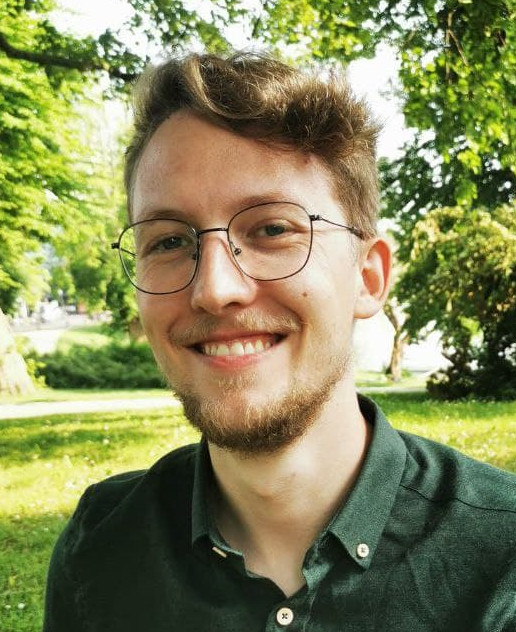
\includegraphics[width=4cm]{media/parkfoto_crop}
	\end{column}
\end{columns}
\end{frame}


\begin{frame}{Context}
I was bored and went looking for a target:
\begin{itemize}
	\item Embedded system to run Doom on
	\item Not too crazy in terms of hardware hacking skills
	\item Cool factor?
\end{itemize}
\end{frame}



\begin{frame}{The device}{VX820}
\centering
\includegraphics[width=10cm]{media/outside_diagonal}
\end{frame}

\begin{frame}{The device}{Why?}
\begin{columns}
	\begin{column}{0.5\textwidth}
		Why a payment terminal?
		\begin{itemize}
			\item Seems unnecessarily powerful
			\item All the useful peripherals
		\end{itemize}
		~

		Why this device?
		\begin{itemize}
			\item Relatively old: easier exploitation?
			\item Still quite common in NL
		\end{itemize}
	\end{column}
	\begin{column}{0.5\textwidth}
		\centering
		% \includegraphics[width=5cm]{media/lcd_testscreen}
		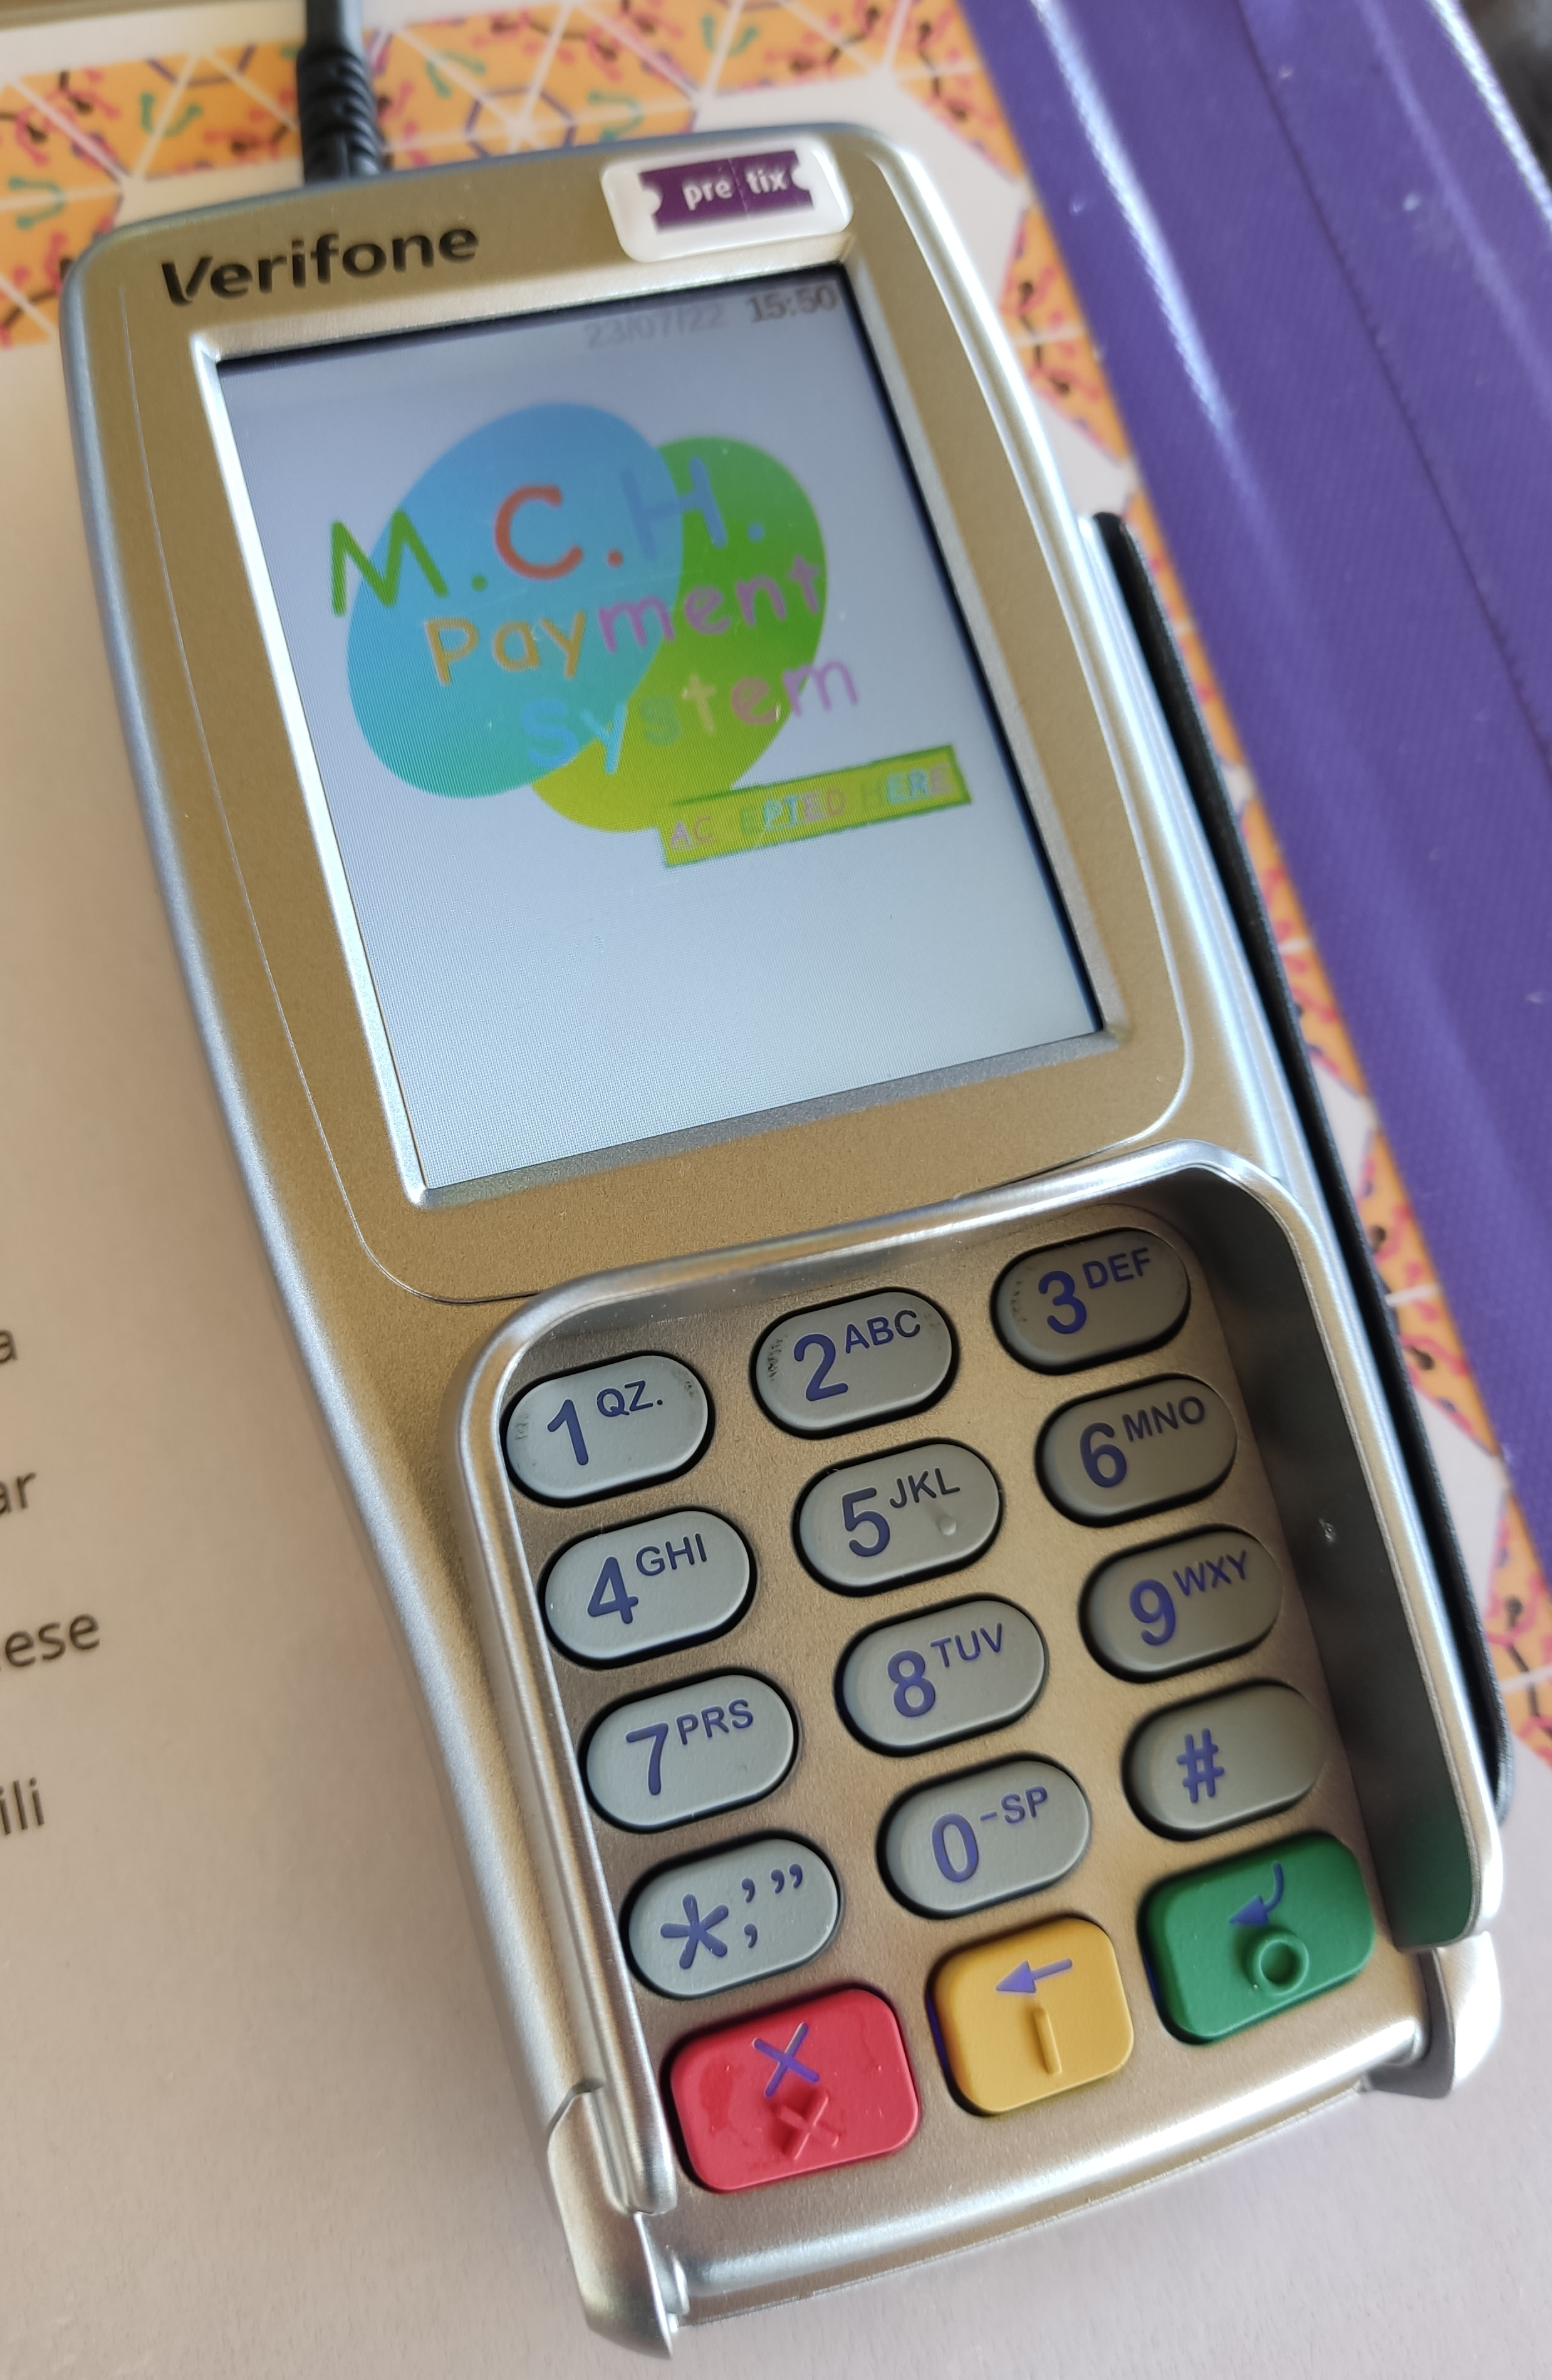
\includegraphics[width=4.7cm]{media/vx820_mch_bar}
	\end{column}
\end{columns}
\end{frame}




% \begin{frame}{The device}{VX820}
% \begin{columns}
% 	\begin{column}{0.5\textwidth}
% 		Verifone VX820
% 		\begin{itemize}
% 			\item 12 years old and (soon to be) discontinued
% 			\item Pin pad or standalone terminal

% 			\item Easy to find on Marktplaats/eBay/...
% 		\end{itemize}
% 	\end{column}
% 	\begin{column}{0.5\textwidth}
% 		\centering
% 		TODO: picture of device at MCH
% 	\end{column}
% \end{columns}
% \end{frame}




\begin{frame}{Device specs}
% \fontsize{11pt}{11pt}\selectfont
\begin{columns}
	\begin{column}{0.5\textwidth}
		Hardware:
		\begin{itemize}
			\item 400Mhz ARMv6 processor
			\item 128MB flash, 32MB RAM
			\item 240x320 color LCD (touchscreen)!
			\item Ethernet, USB, serial
			\item Smartcard reader (x4), NFC, magstripe, beeper
		\end{itemize}
		Software:
		\begin{itemize}
			\item "Verix OS"
			\item Multi-application
			\item Configuration through env vars
			\item Unix-like filesystem/syscalls
		\end{itemize}
	\end{column}
	\begin{column}{0.5\textwidth}
		\centering
		\includegraphics[width=6cm]{media/lcd_boot}
	\end{column}
\end{columns}
\end{frame}

\begin{frame}
\begin{columns}
	\begin{column}{0.5\textwidth}
		\centering
		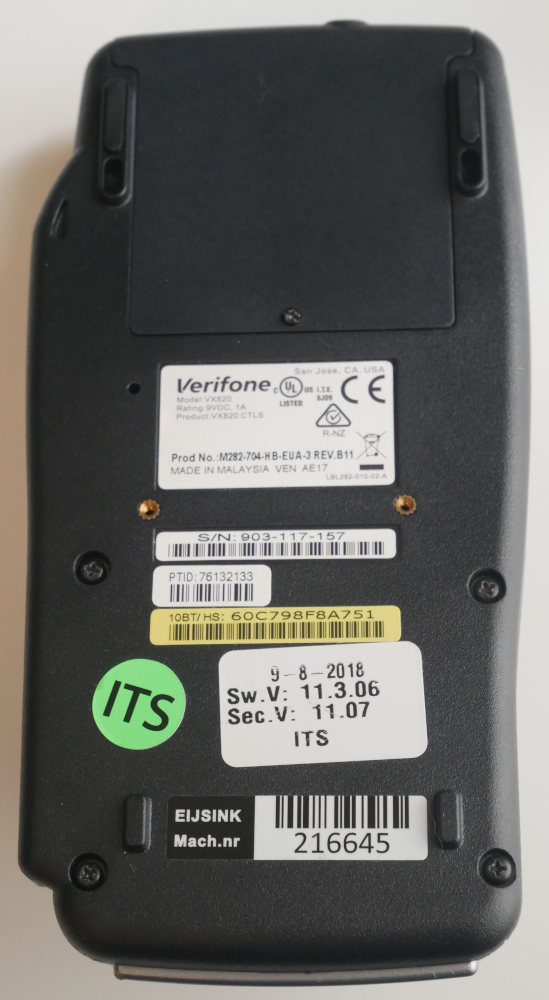
\includegraphics[width=5cm]{media/outside_bottom}	
	\end{column}
	\begin{column}{0.5\textwidth}
		\centering
		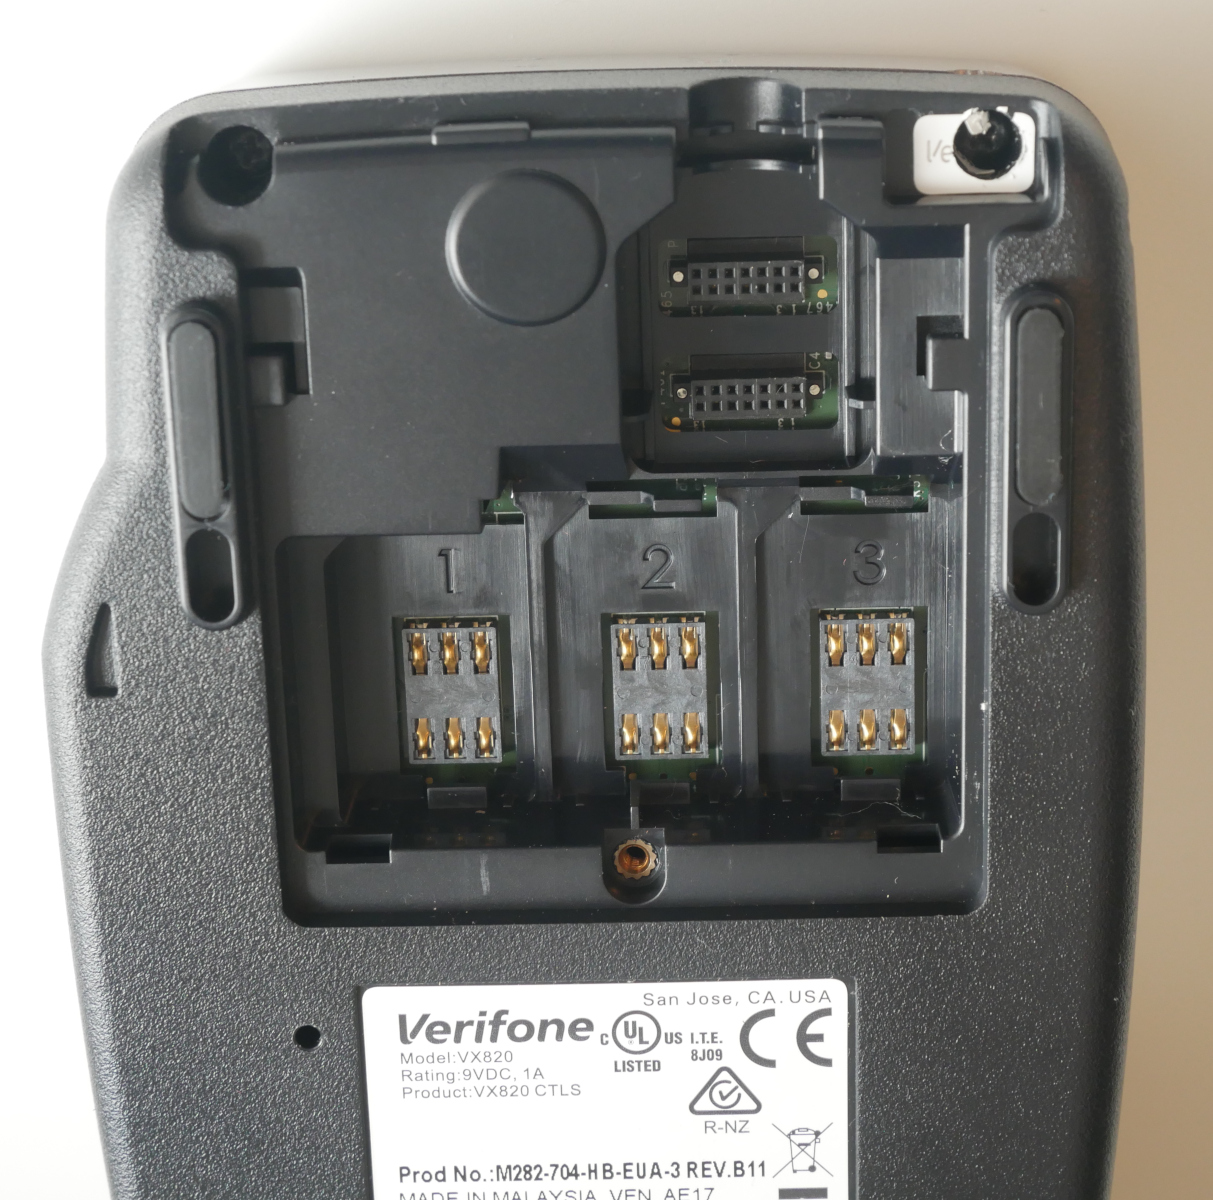
\includegraphics[width=7cm]{media/outside_bottom_under_flap}
	\end{column}
\end{columns}
\end{frame}


% TODO: arrows pointing to interesting areas/components?
\begin{frame}
\centering
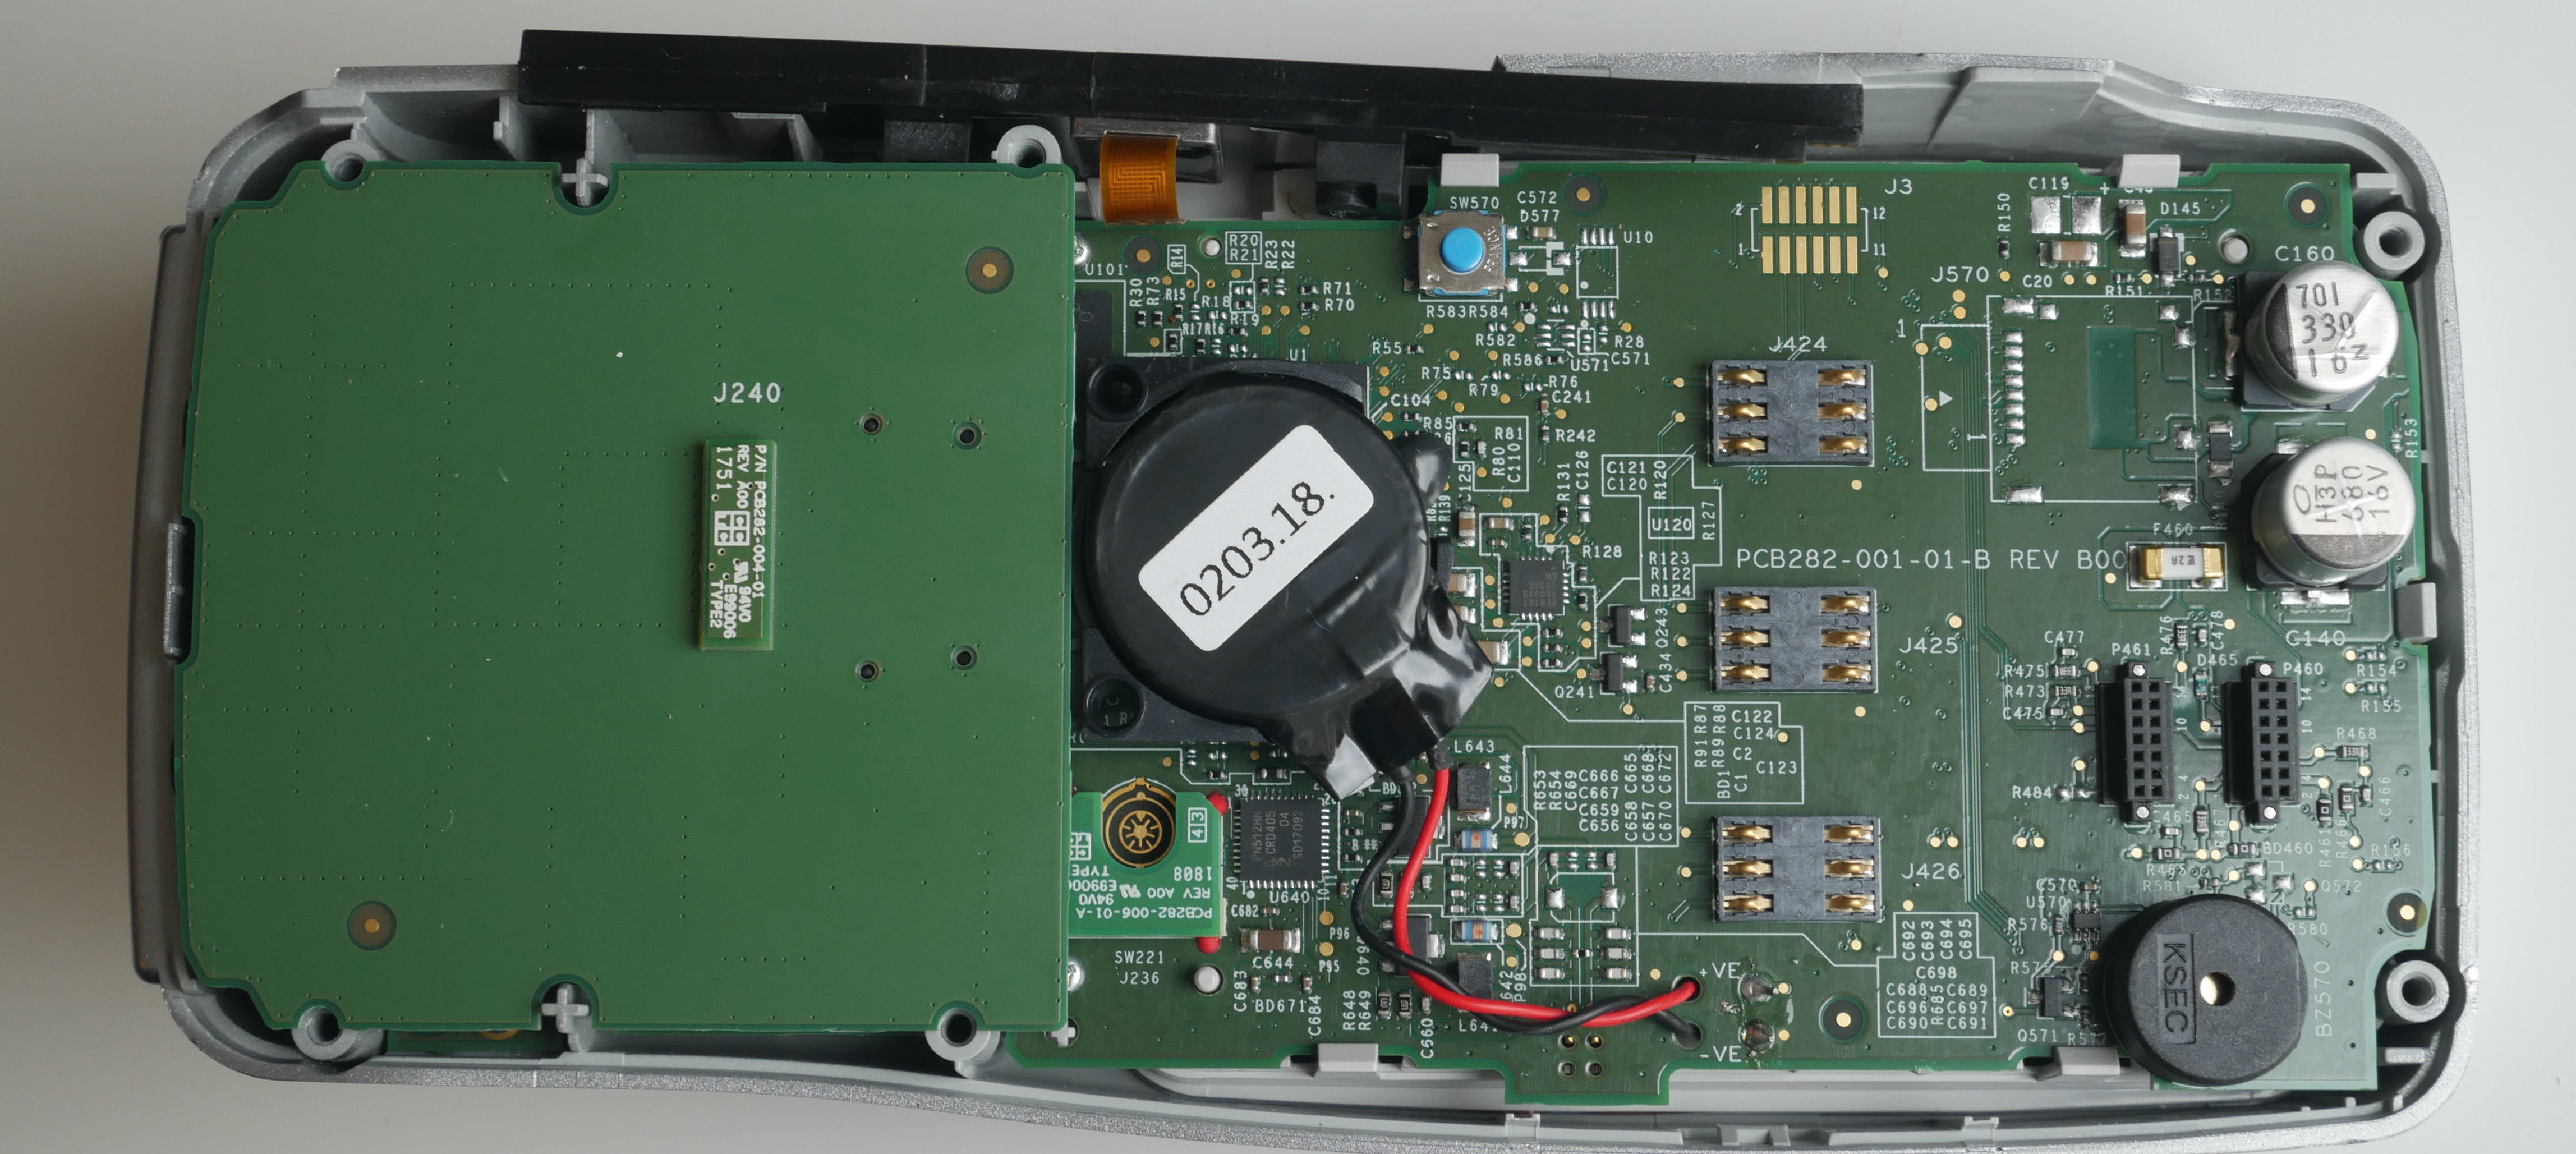
\includegraphics[width=14cm]{media/pcb}
\end{frame}

\begin{frame}
\centering
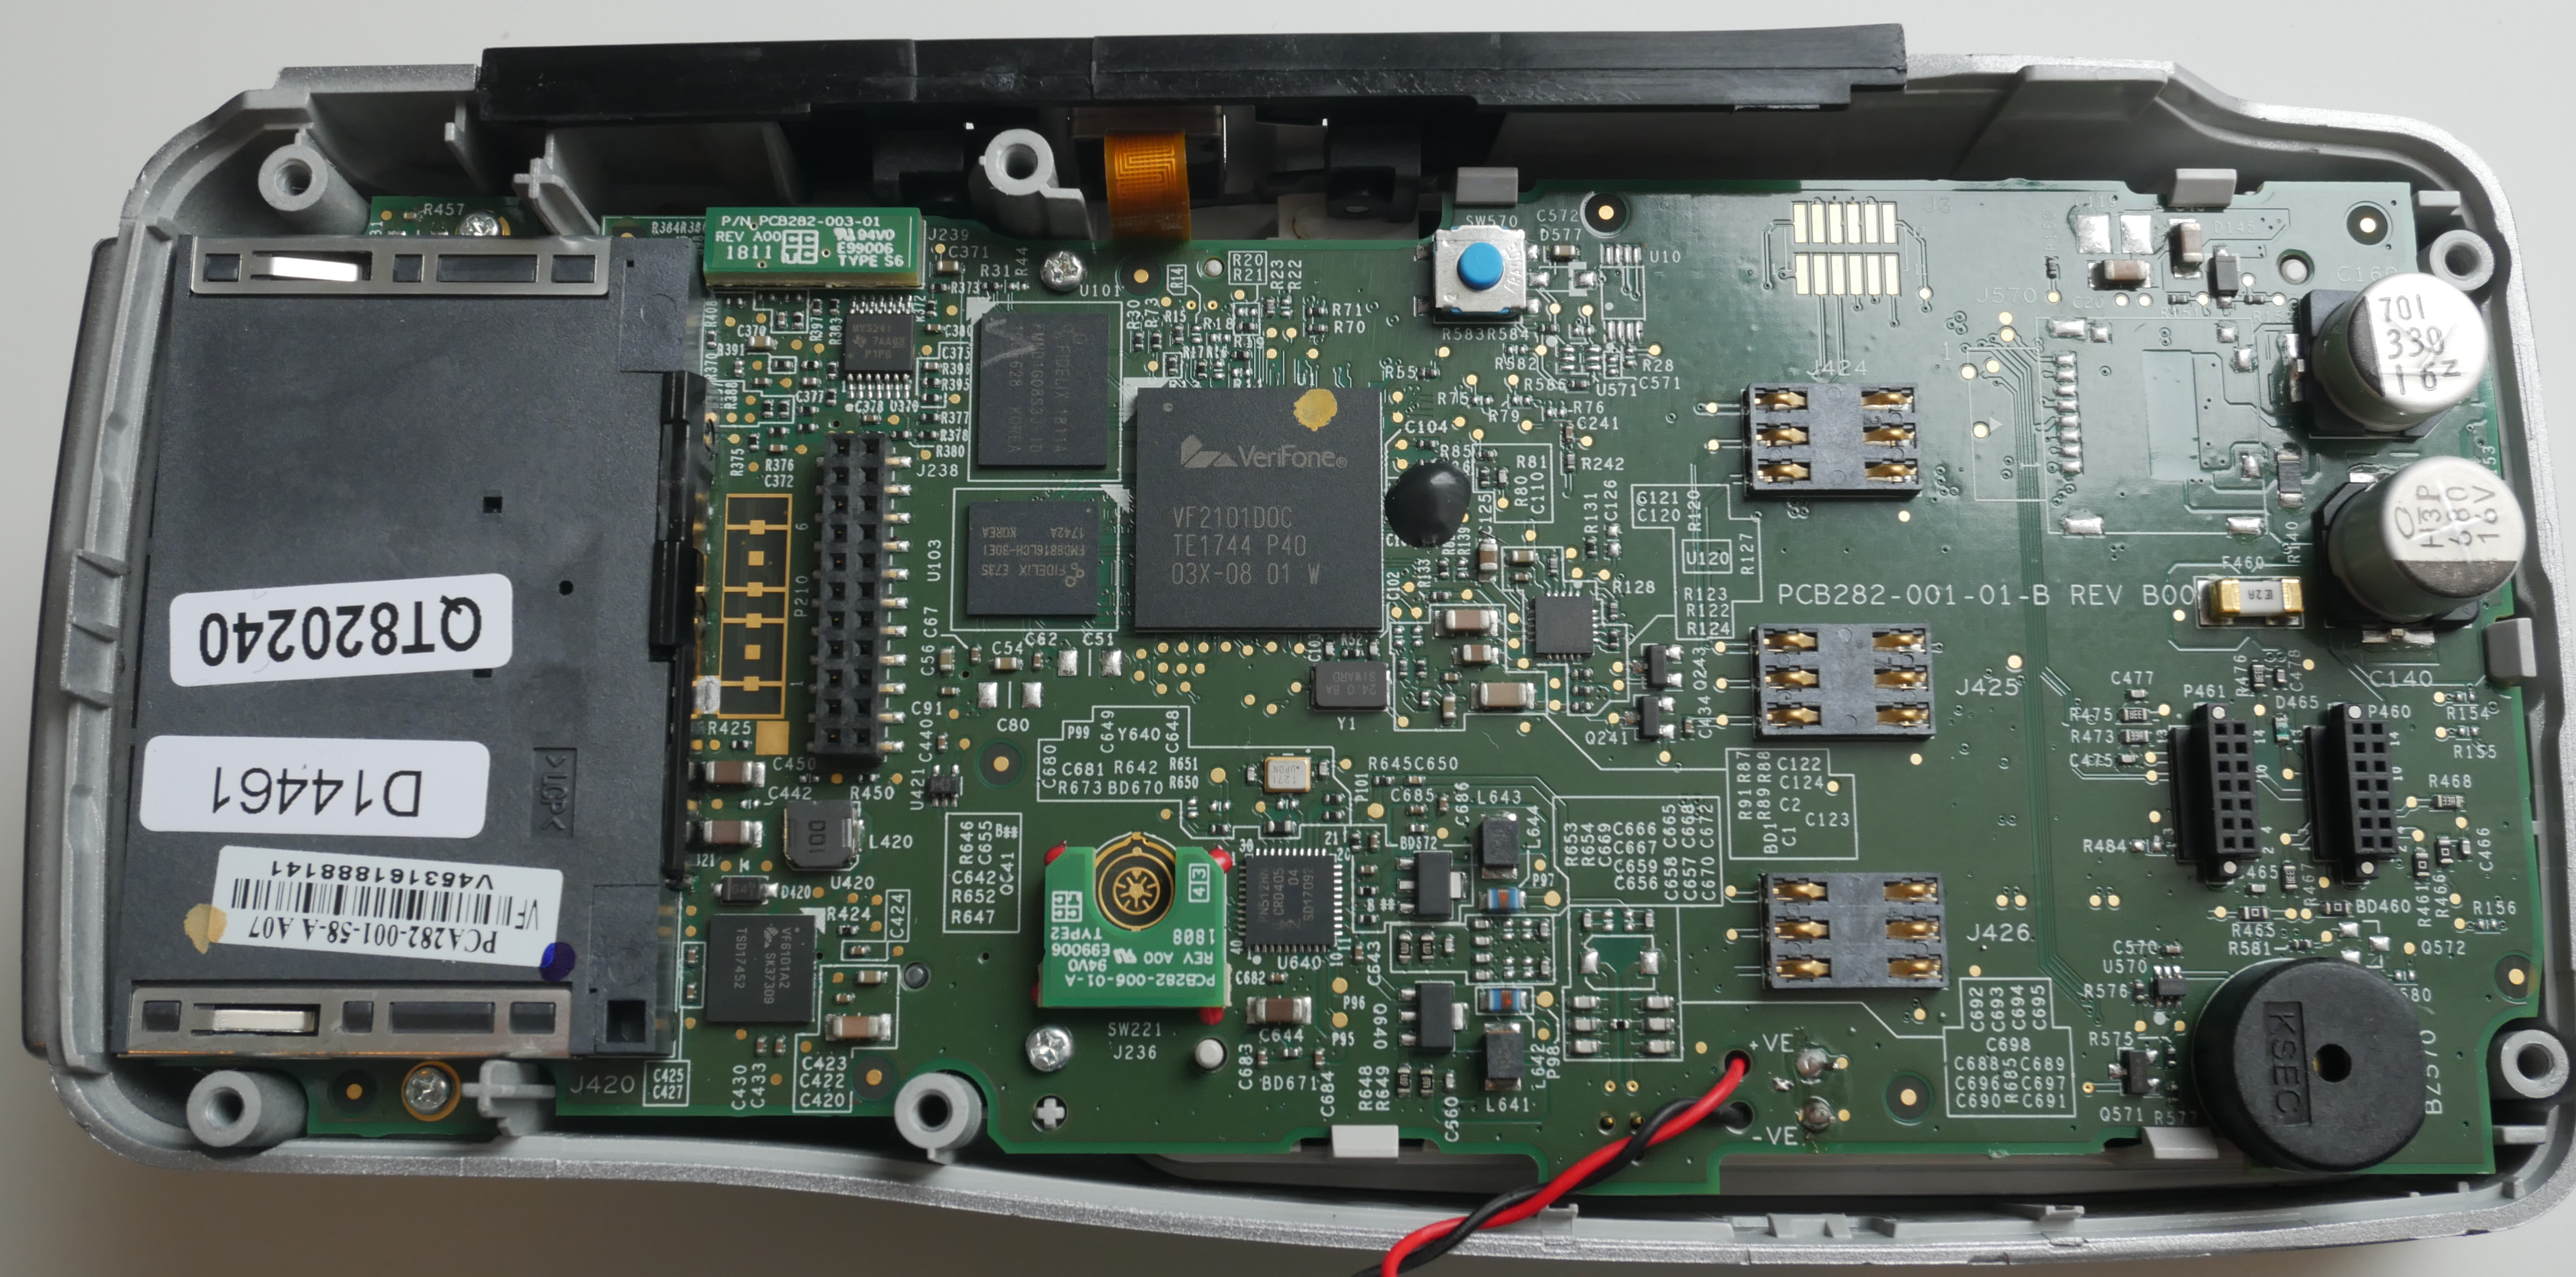
\includegraphics[width=14cm]{media/pcb_noshield}
\end{frame}

\begin{frame}
\centering
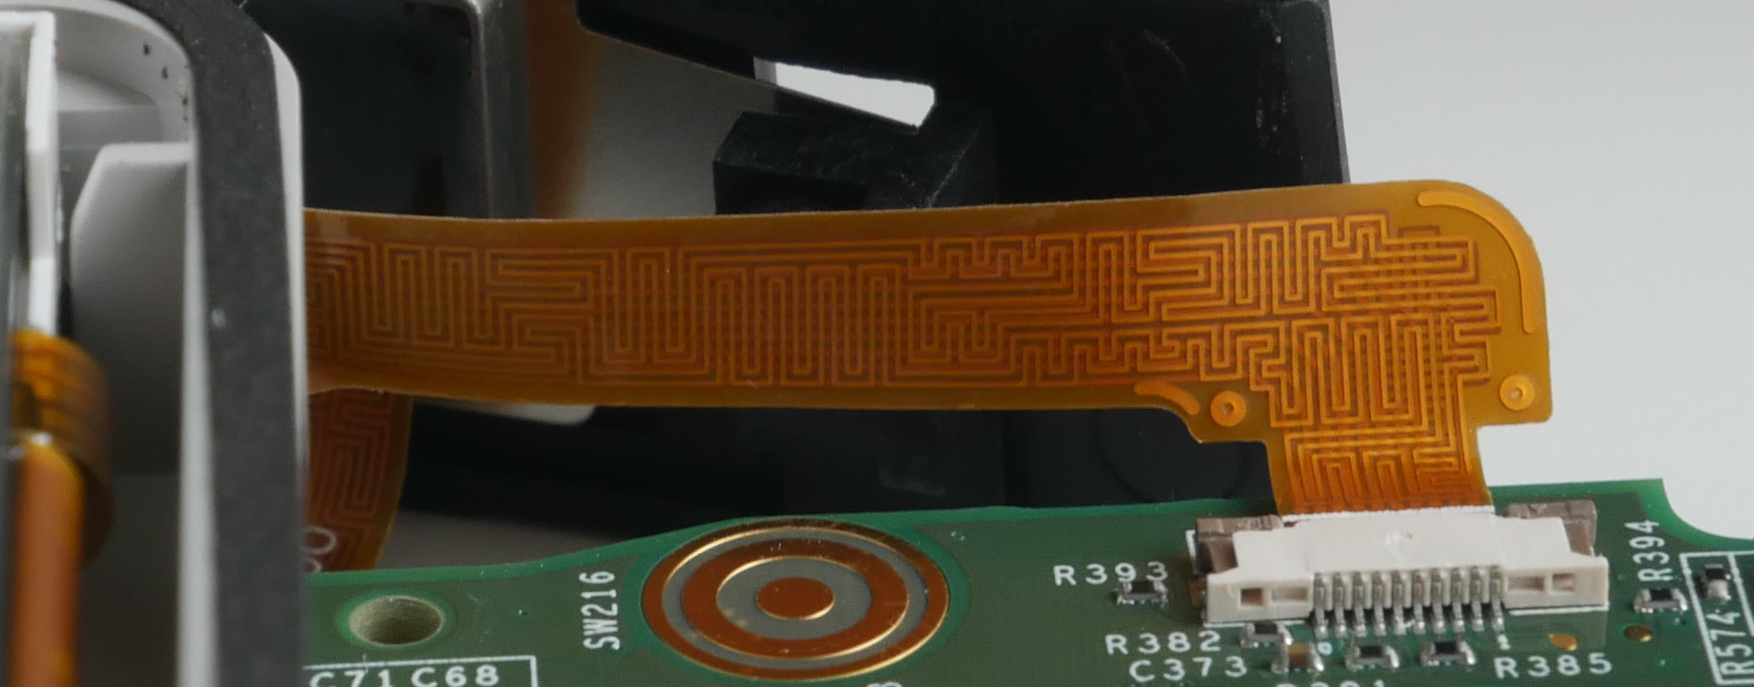
\includegraphics[width=12cm]{media/magstripe_connector3_crop}
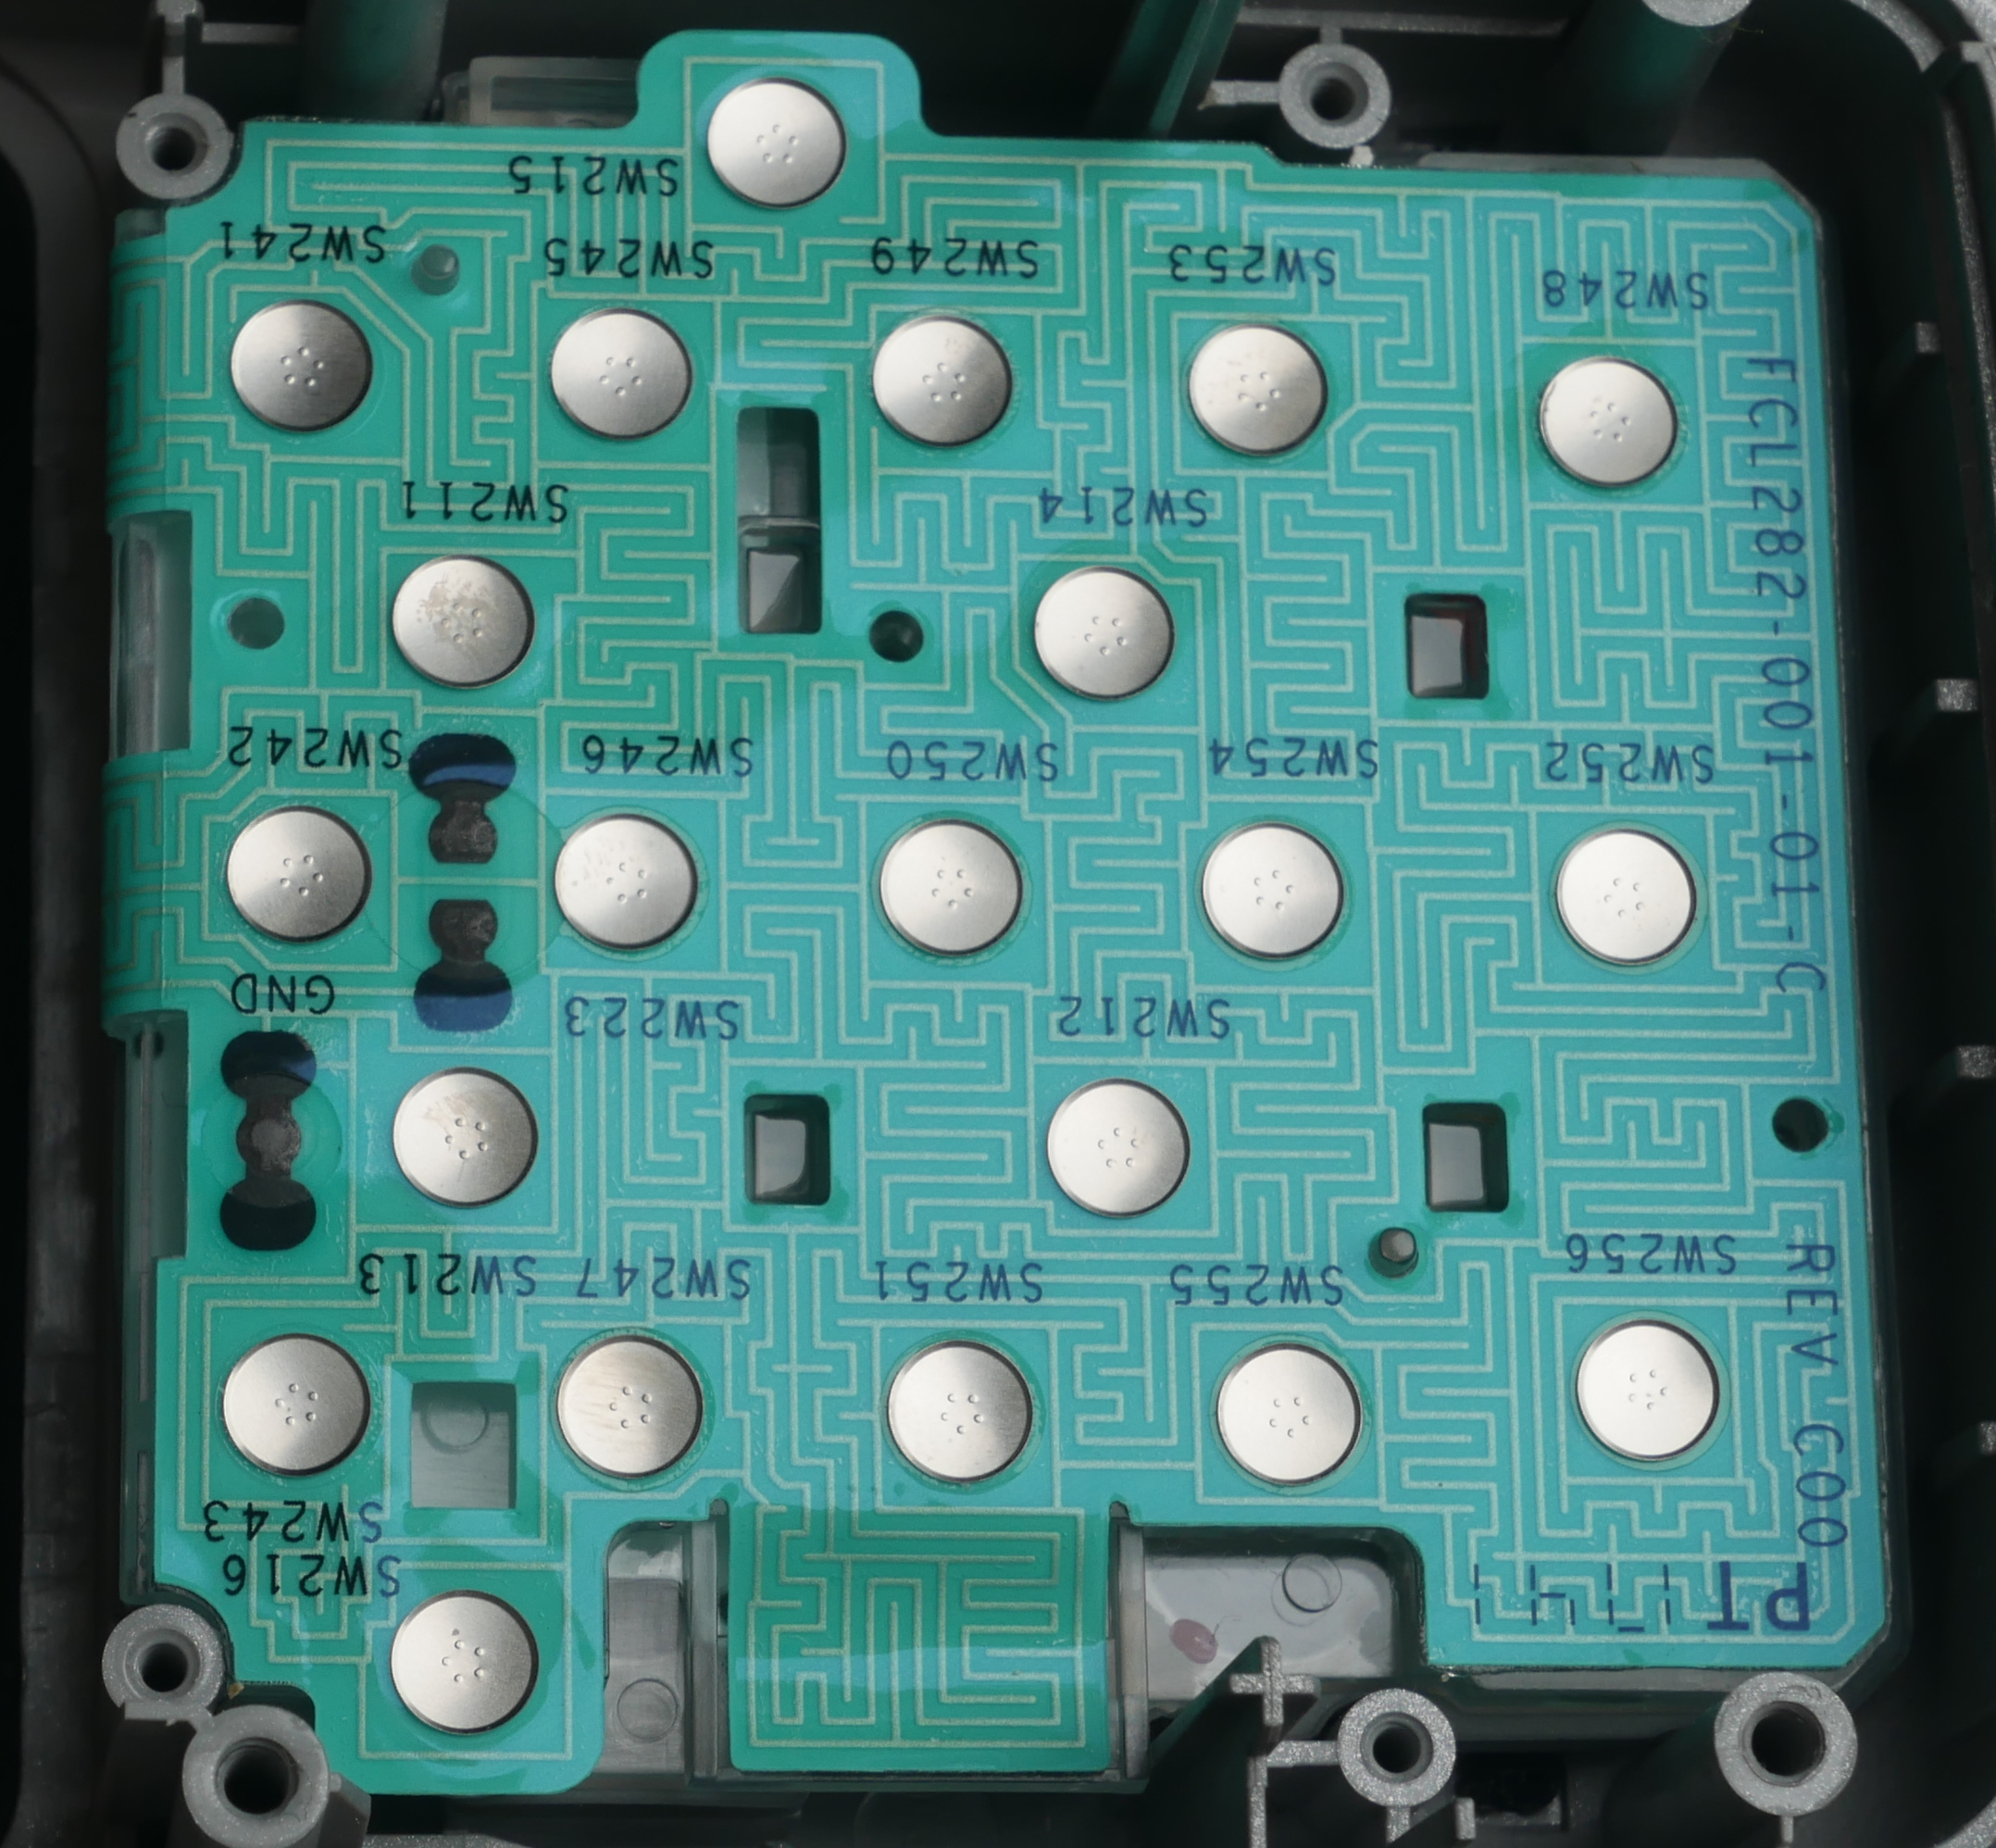
\includegraphics[width=7.5cm]{media/pinpad_squigglies}
\end{frame}

\begin{frame}
\centering
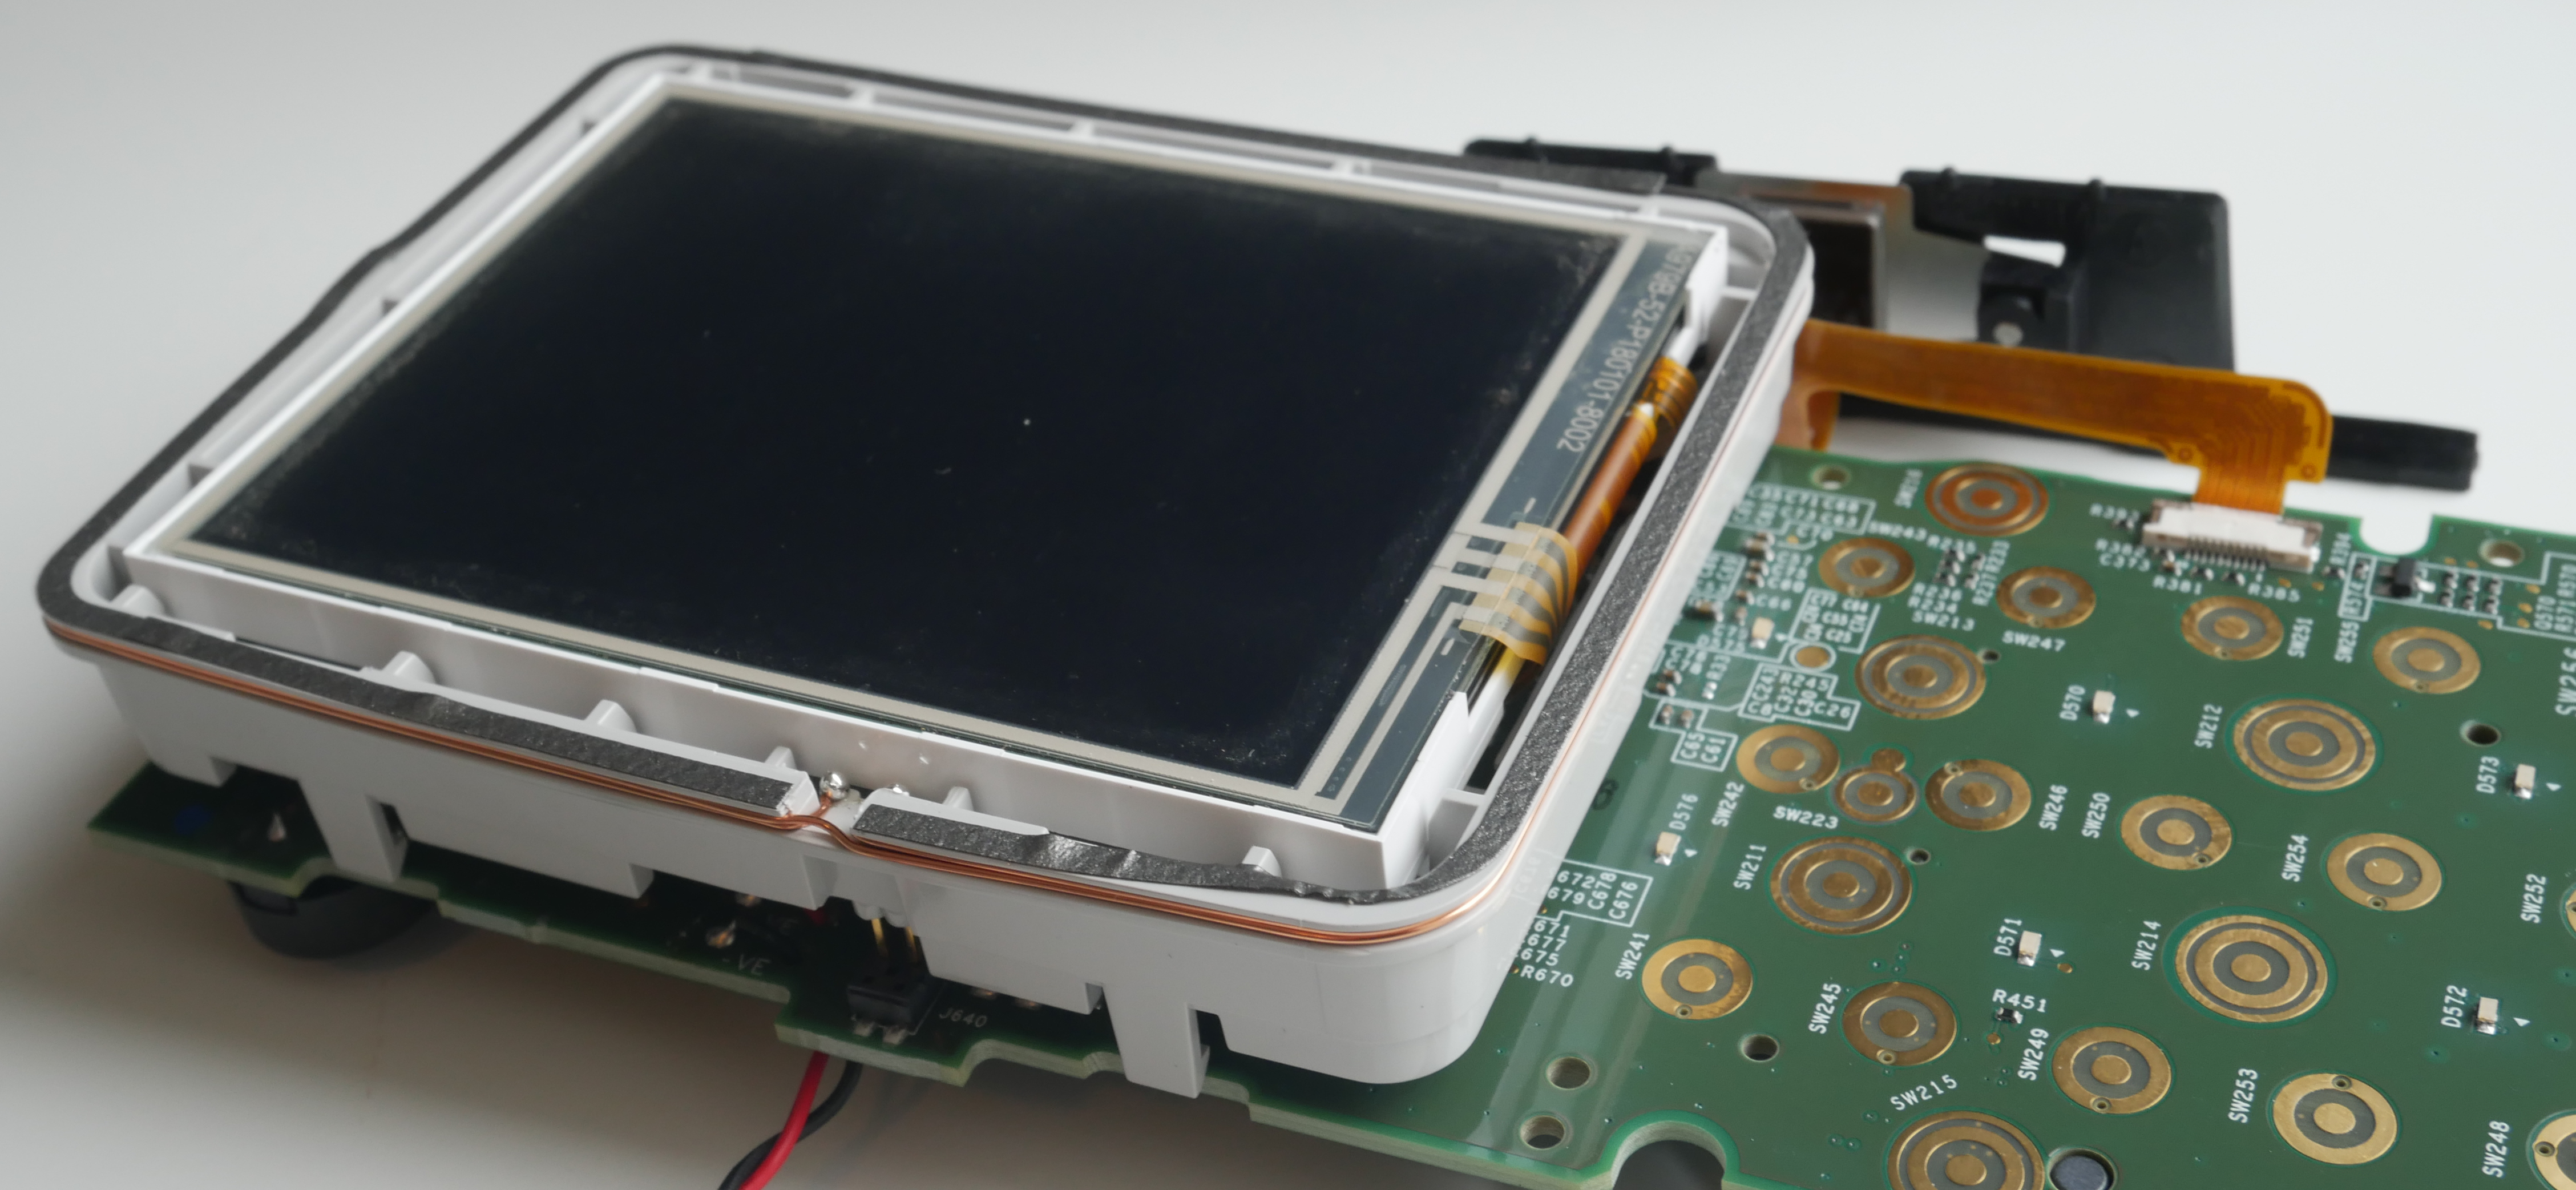
\includegraphics[width=14cm]{media/screen_coil}
\end{frame}

\begin{frame}
\centering
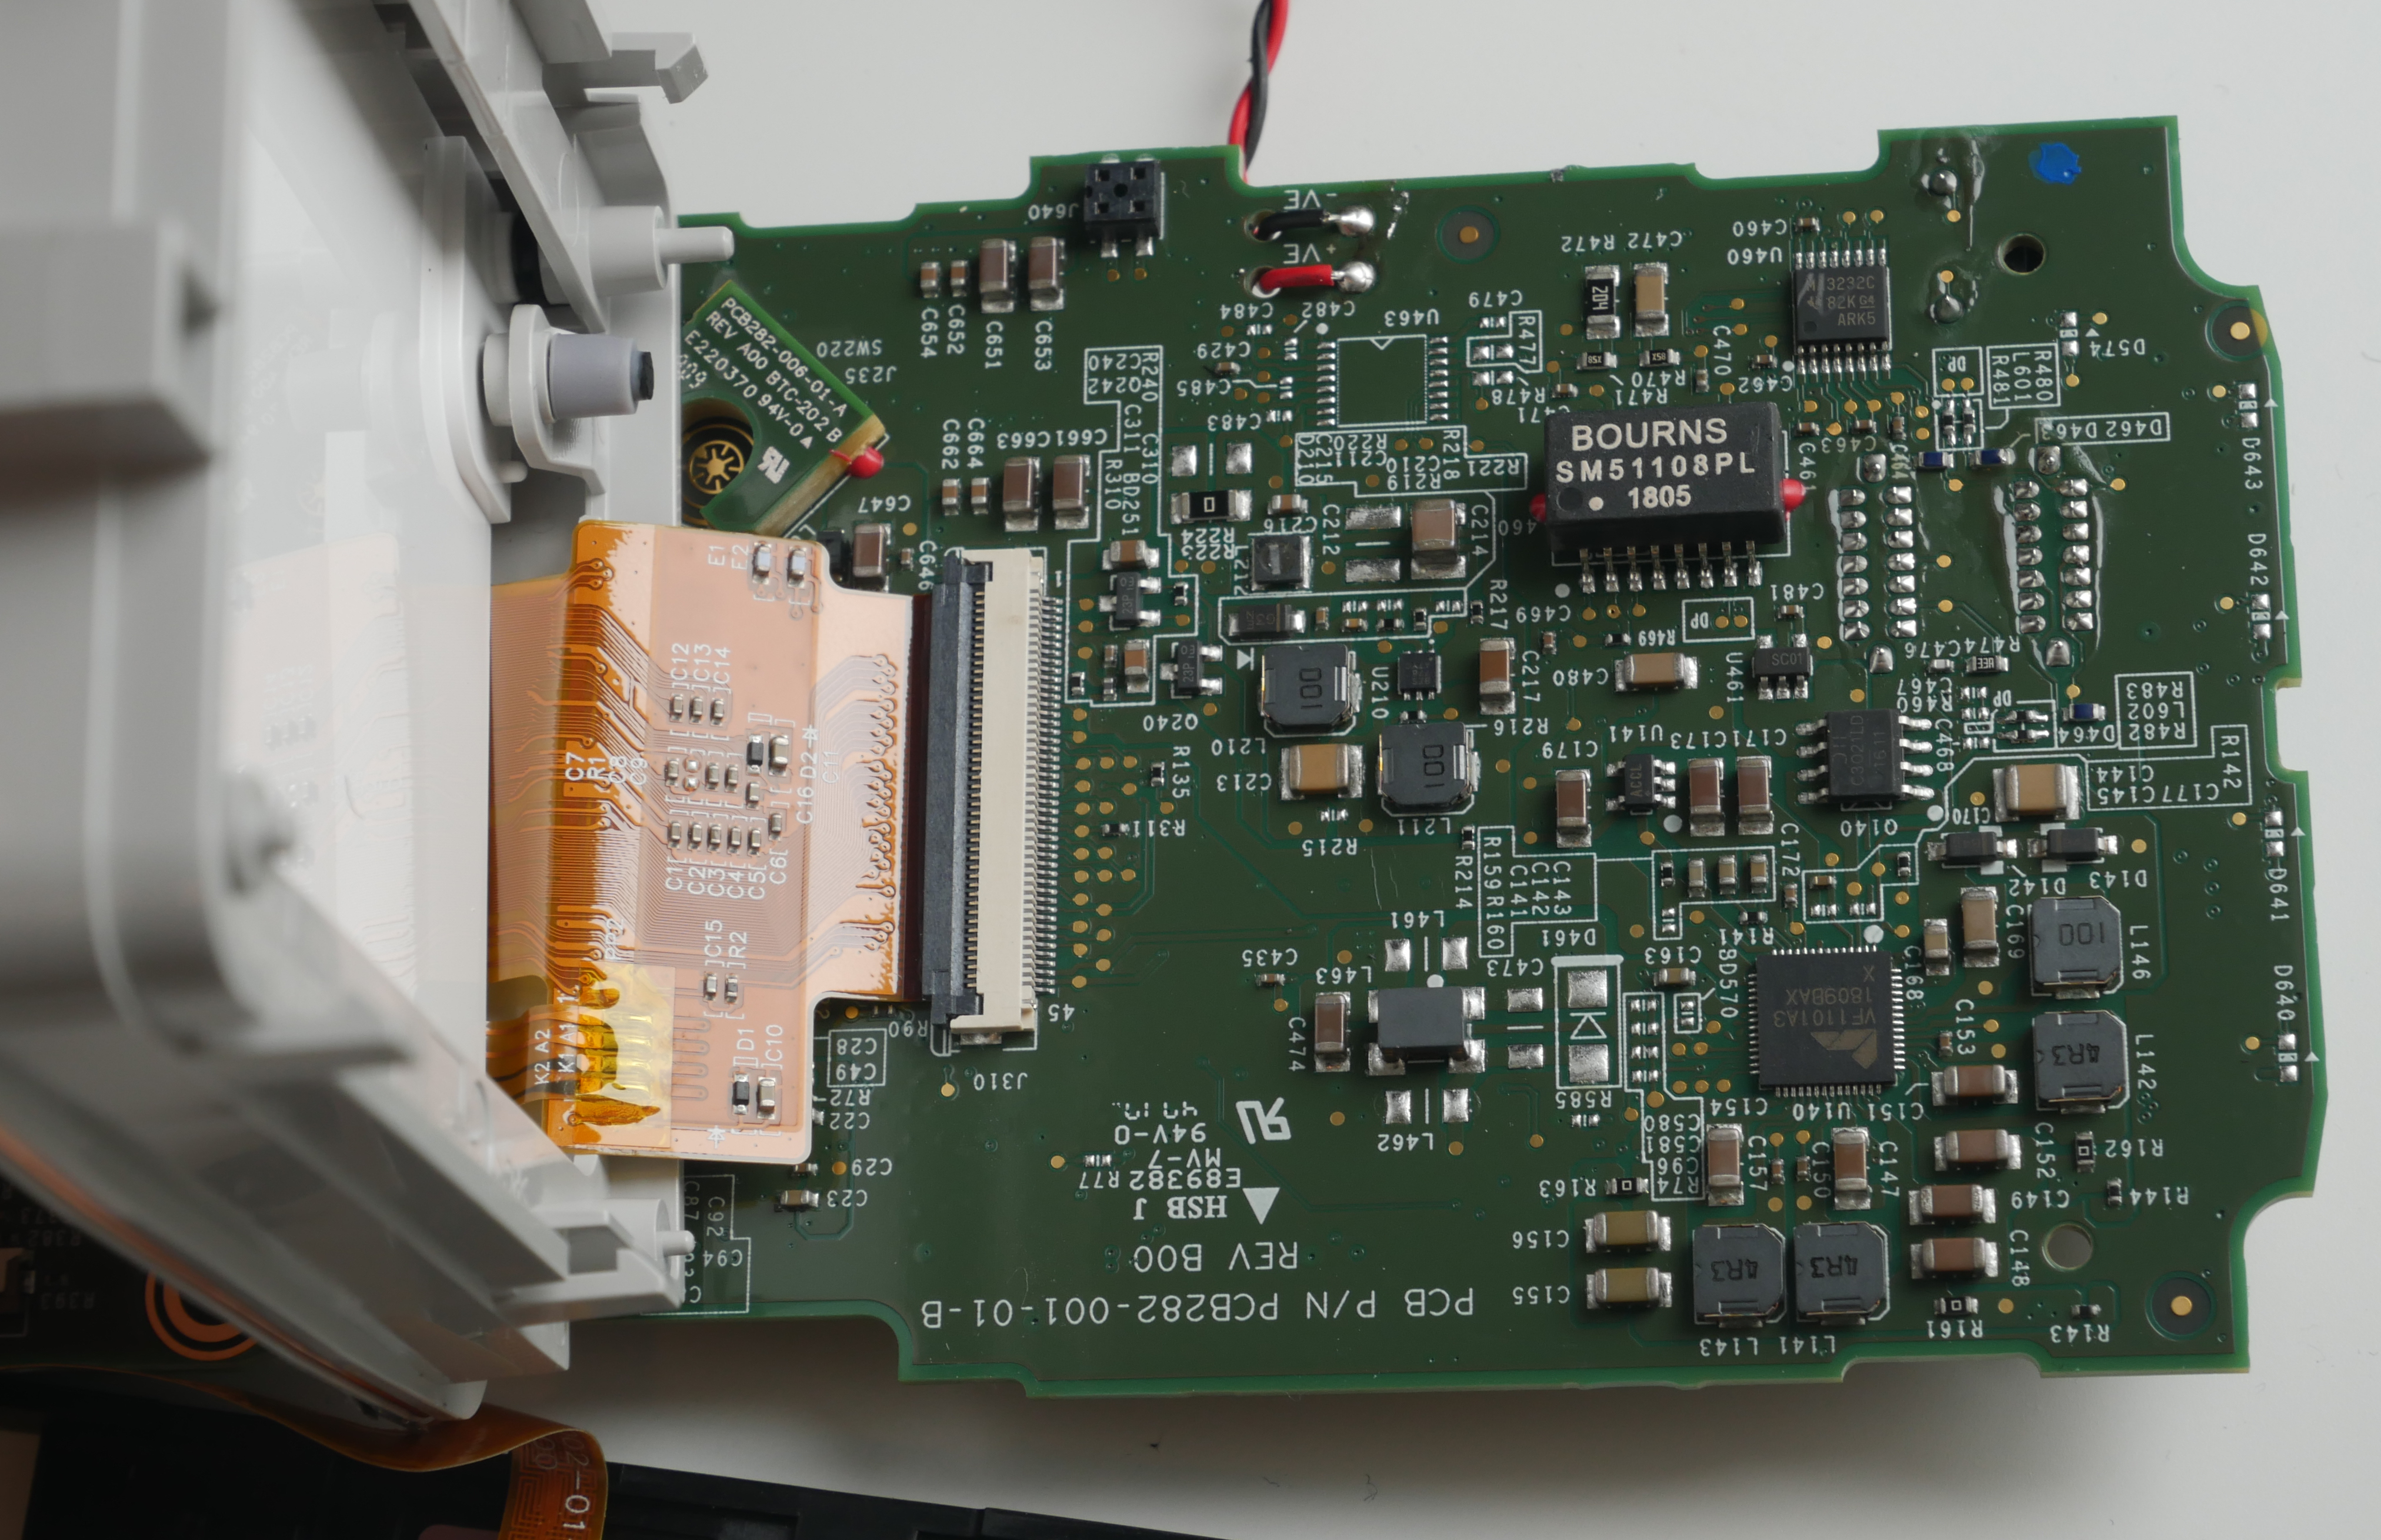
\includegraphics[width=14cm]{media/pcb_under_screen}
\end{frame}


% time here: 18min
\begin{frame}{Getting access}{How it all began}
\centering
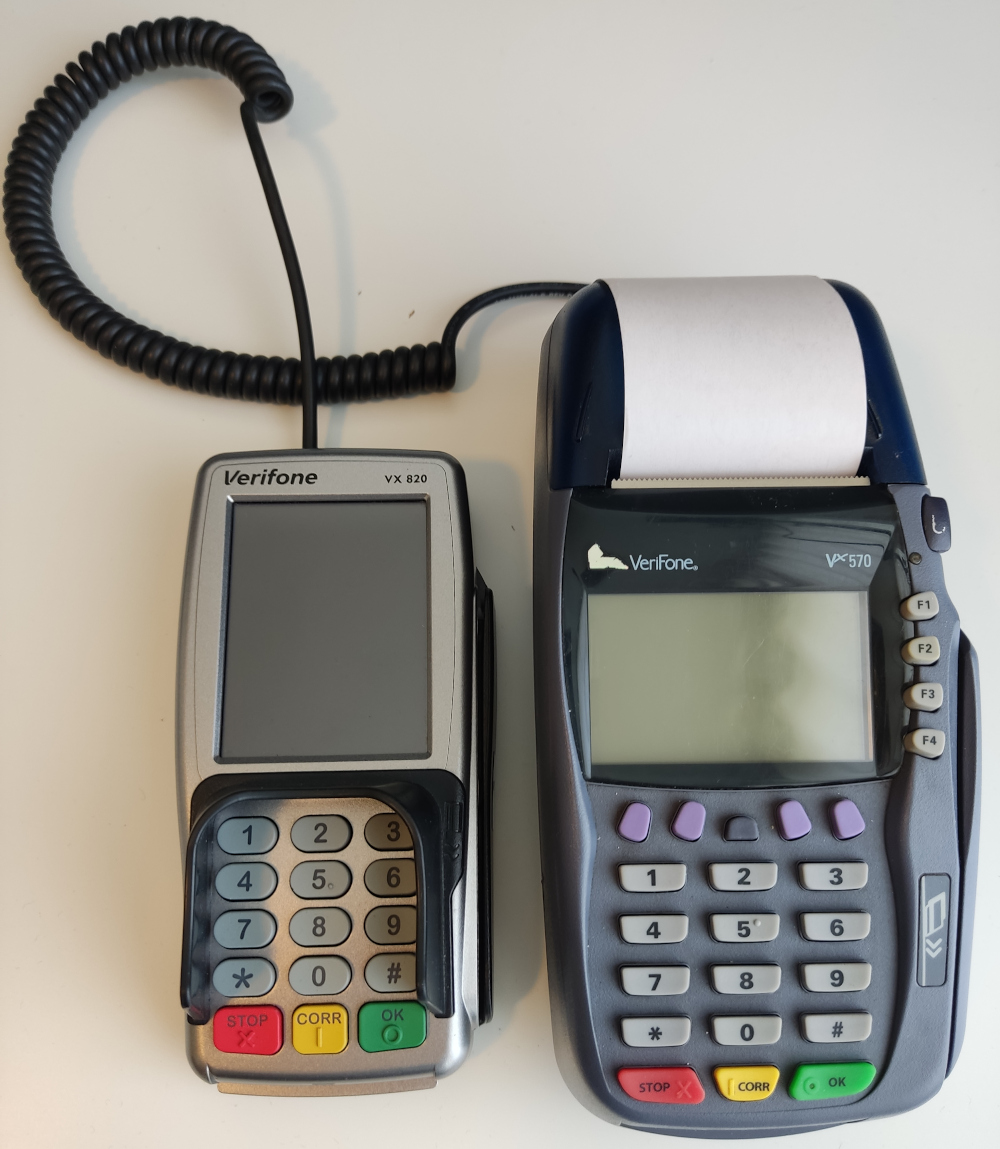
\includegraphics[width=6cm]{media/vx820_with_vx570}
\end{frame}



\begin{frame}{Getting access}
Initial state:
\begin{itemize}
	\item Running the CCV payment application
	\item Configured as a ``pin pad''
\end{itemize}

~

Locked down..
\begin{itemize}
	\item No way to exit application
	\item System menu shortcut disabled
	\item Only processing commands from POS
\end{itemize}
\end{frame}


\begin{frame}{Getting access}{Capturing the commands between the VX570 and the VX820}
	\centering
	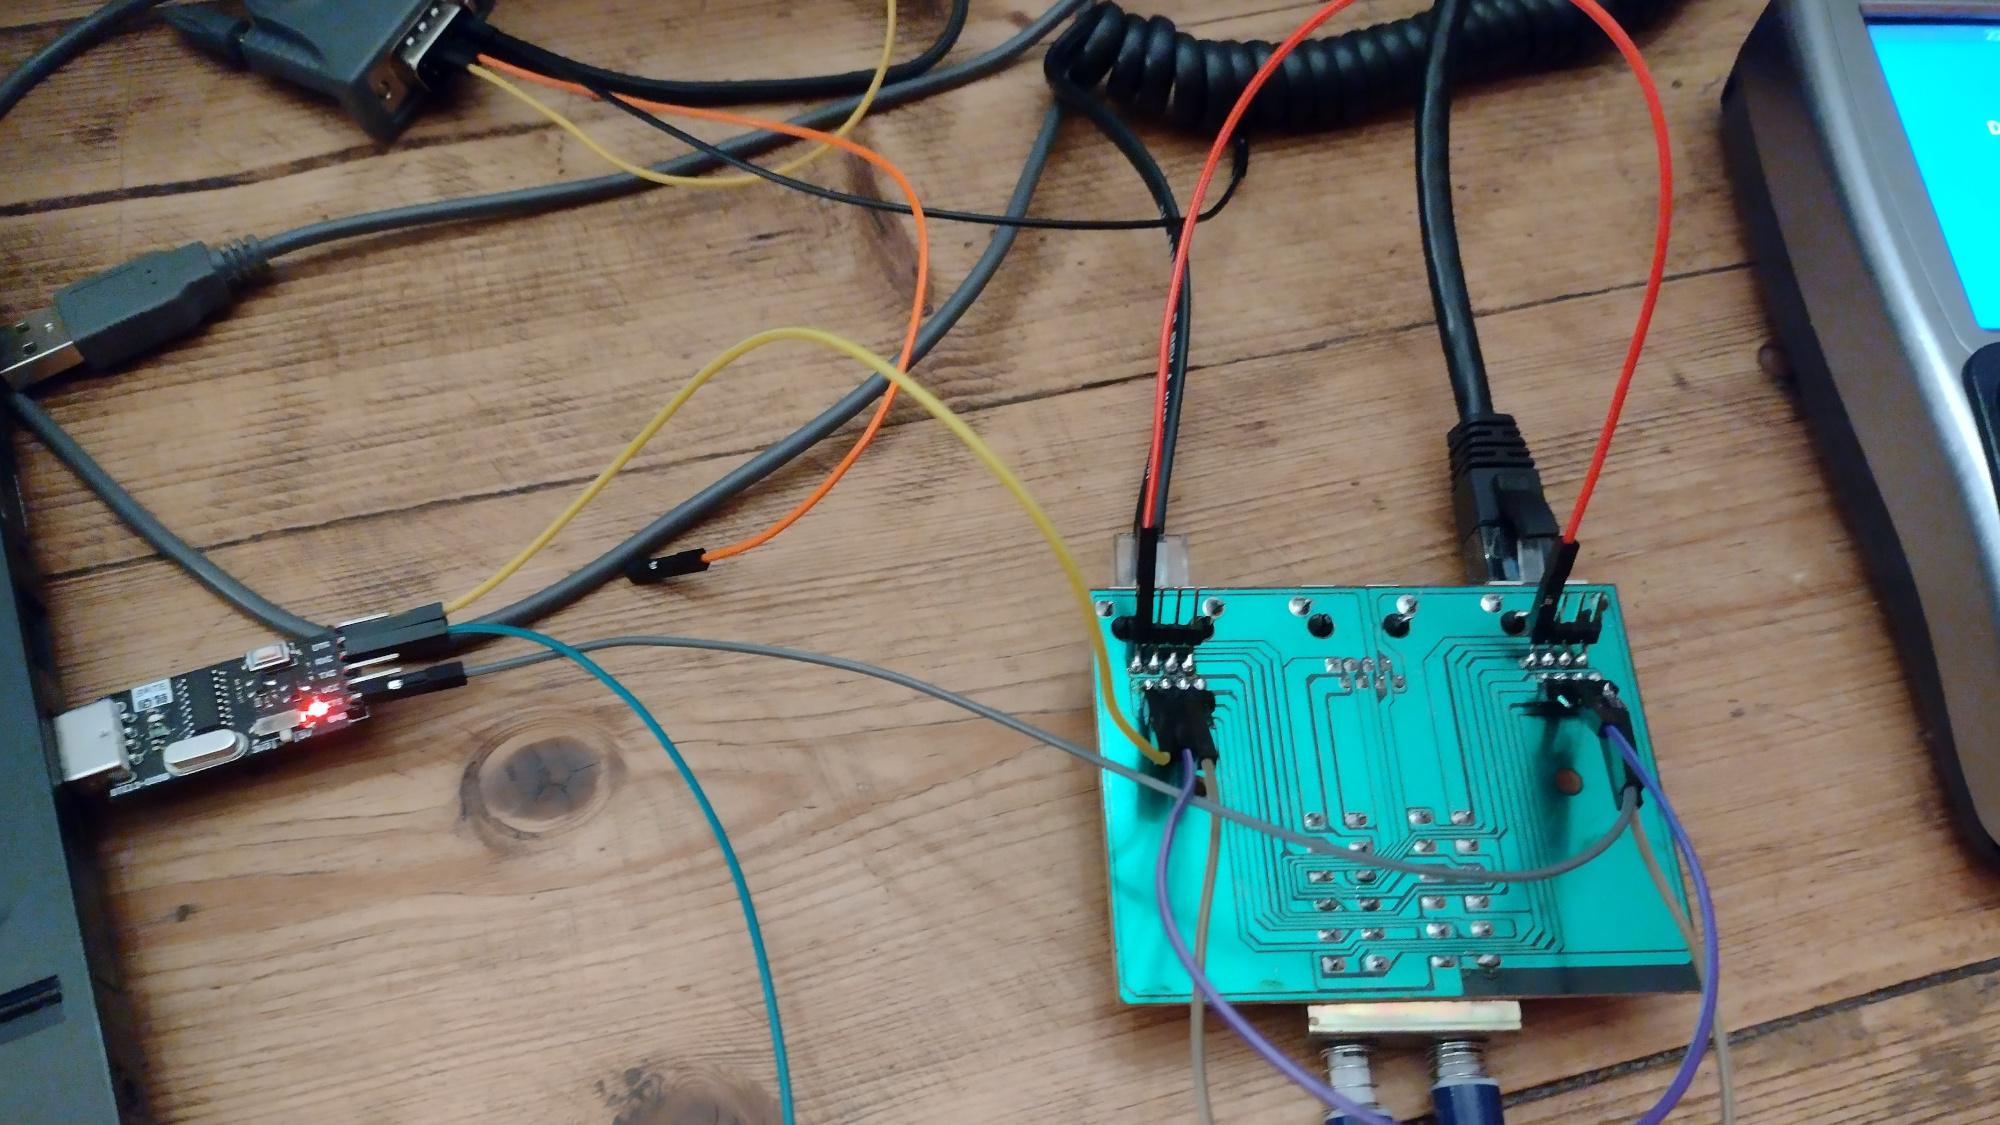
\includegraphics[width=0.9\textwidth]{media/intercept_serial}
\end{frame}

\begin{frame}{Getting access}{Some time later :)}
	\centering
	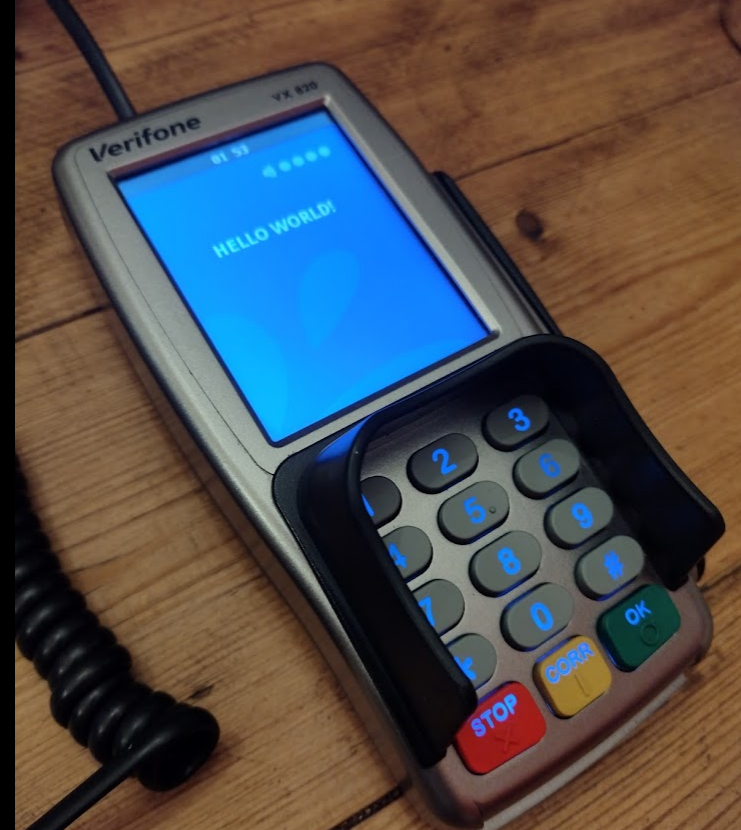
\includegraphics[width=8cm]{media/ccv_hello_world}
\end{frame}


\begin{frame}{Getting access}
	But this doesn't get us any closer to Doom...
\end{frame}


\begin{frame}{Getting access}
	These devices wipe sensitive data when tampered with.

	~

	So what happens when we open it up?
\end{frame}


% \begin{frame}{Getting access}{A different screen!}
% \centering
% 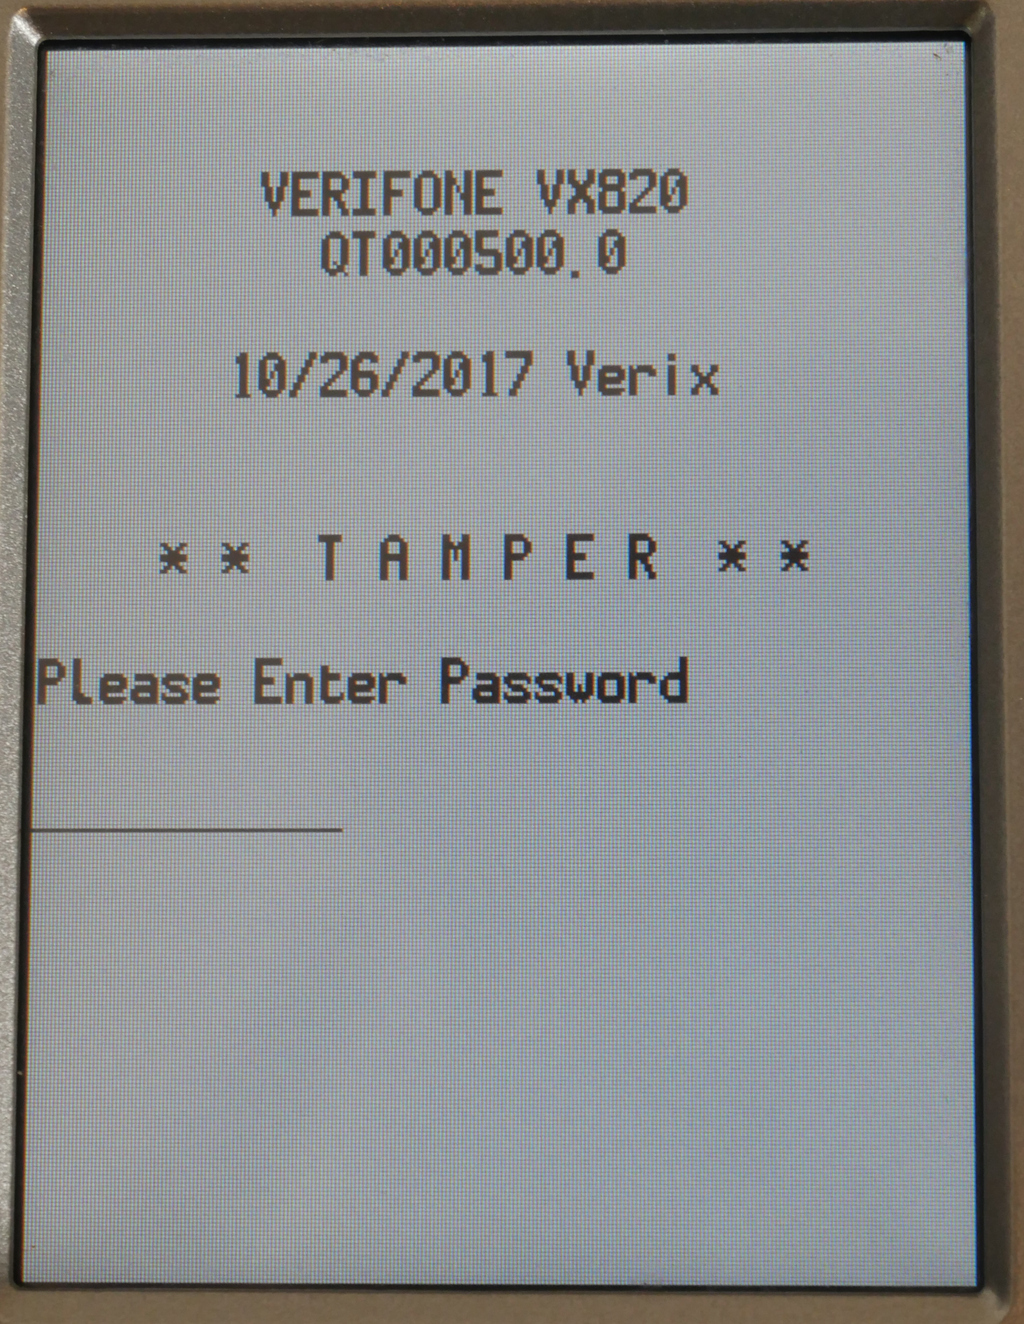
\includegraphics[width=5.5cm]{media/lcd_tamper1}
% \end{frame}


\begin{frame}{Getting access}{A different screen!}
\begin{columns}
	\begin{column}{0.5\textwidth}
		\begin{itemize}
			\item Device is fully wiped
			\item Now boots into system menu
		\end{itemize}
		~

		System menu password is publicly documented :)
		\only<2>{\\~\\\textbf{166831}}
	\end{column}
	\begin{column}{0.5\textwidth}
		\centering
		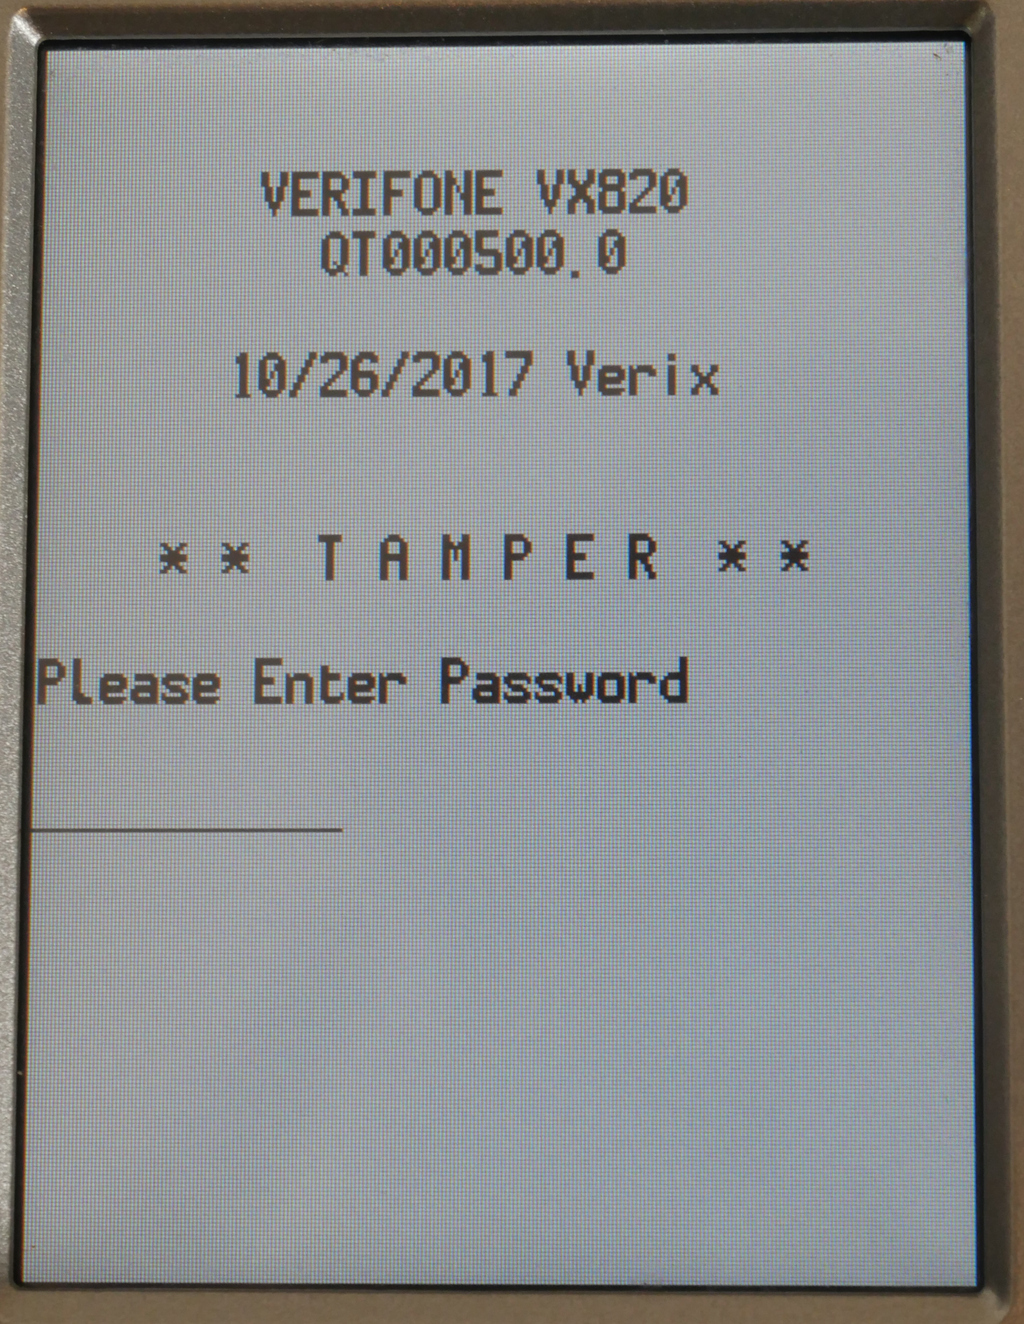
\includegraphics[width=5.5cm]{media/lcd_tamper1}
	\end{column}
\end{columns}
\end{frame}




\begin{frame}{Clearing the tamper flag}
\centering
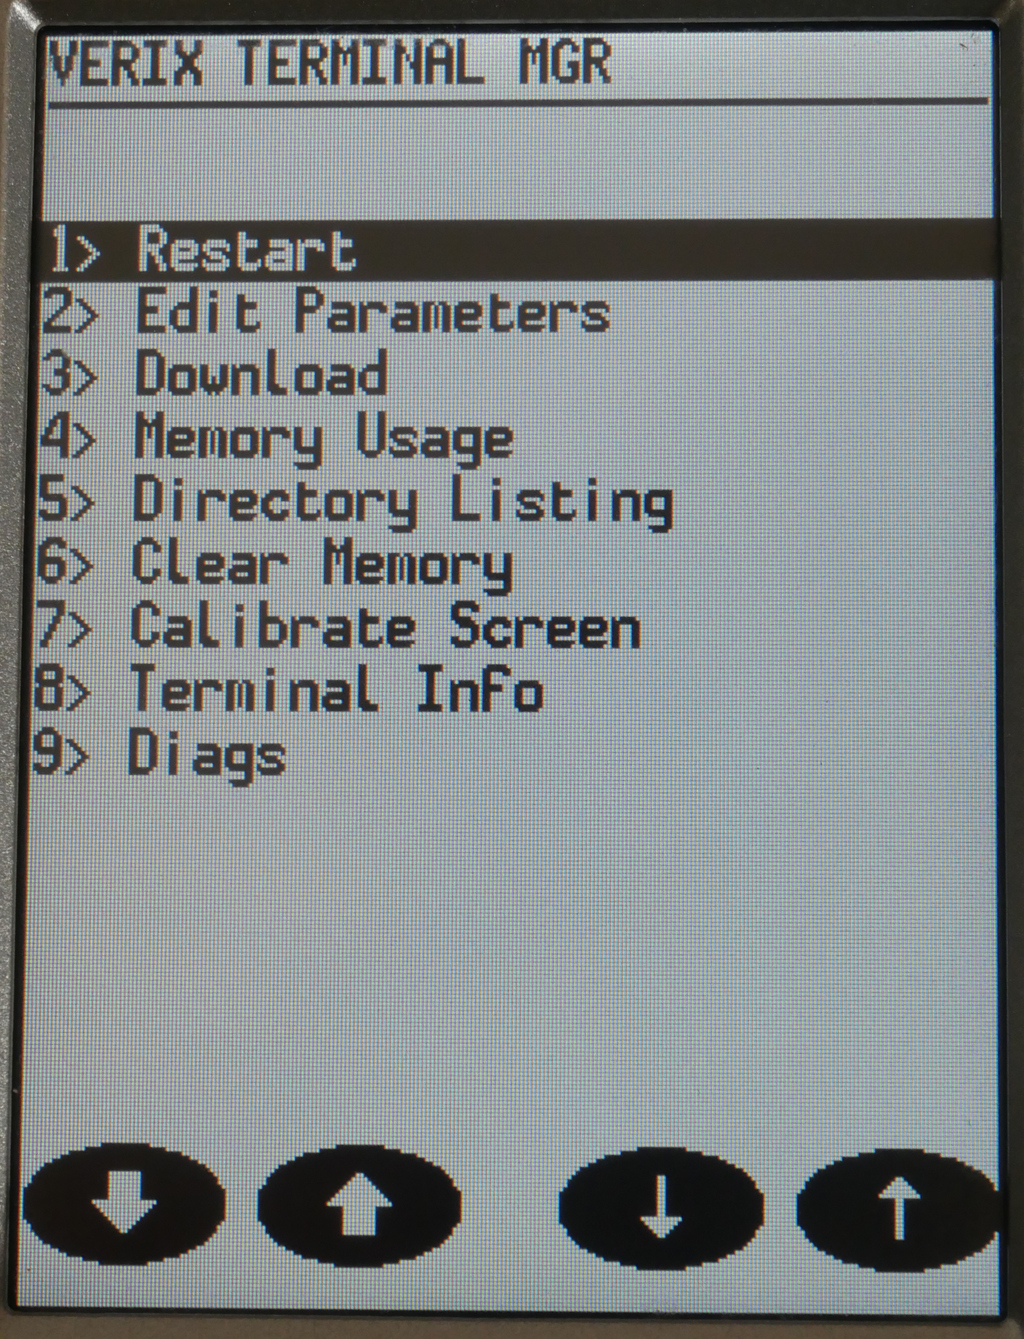
\includegraphics[width=5.5cm]{media/lcd_tamper2}
\end{frame}

\begin{frame}{Clearing the tamper flag}
\centering
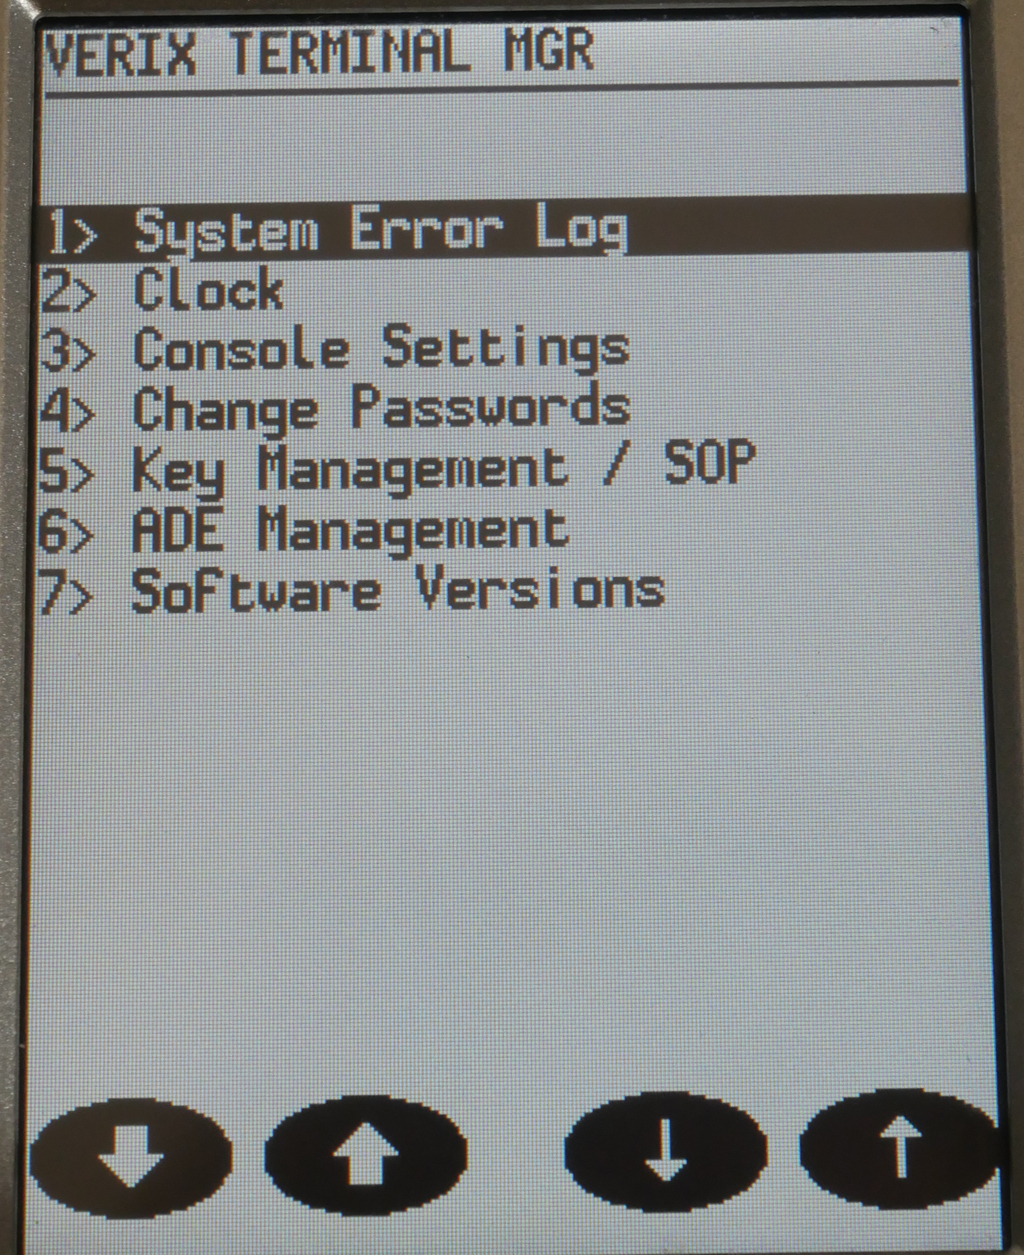
\includegraphics[width=5.5cm]{media/lcd_tamper3}
\end{frame}

\begin{frame}{Clearing the tamper flag}
\centering
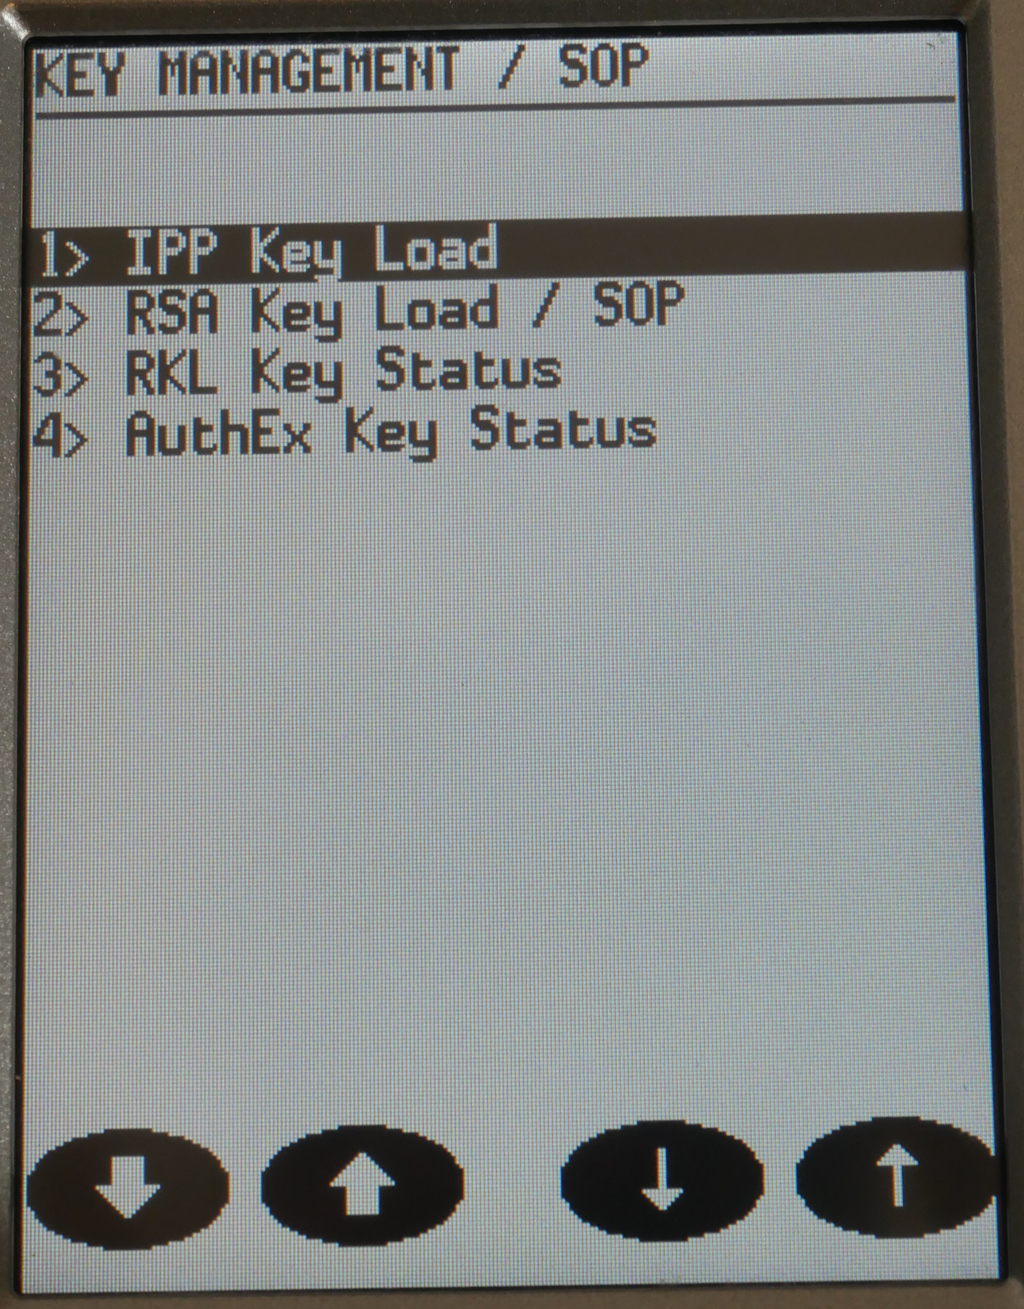
\includegraphics[width=5.5cm]{media/lcd_tamper5}
\end{frame}

\begin{frame}{Clearing the tamper flag}
\centering
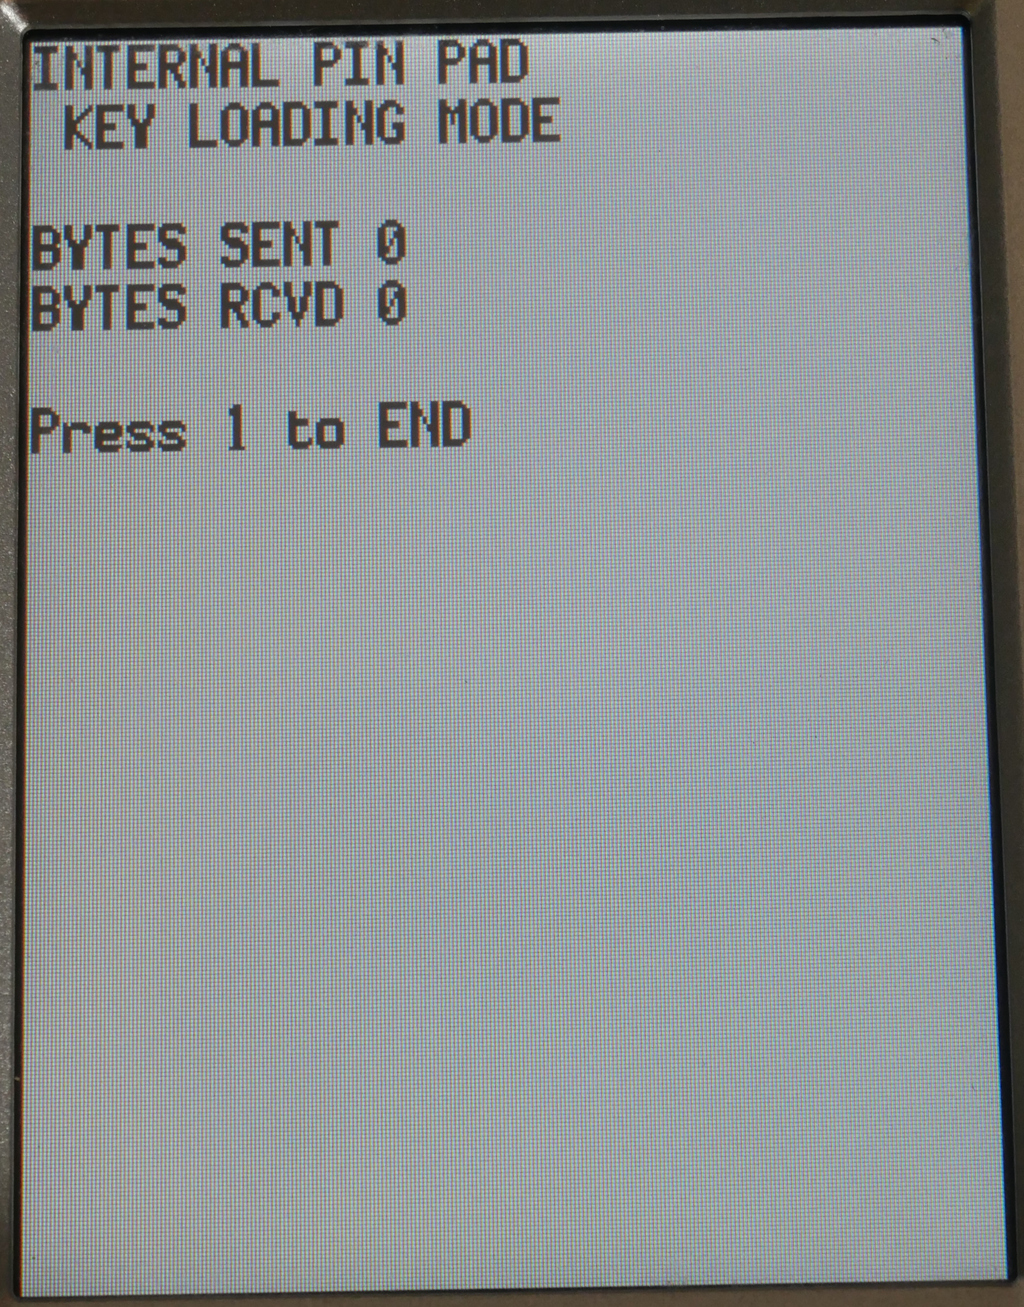
\includegraphics[width=5.5cm]{media/lcd_tamper6}
\end{frame}

\begin{frame}{Clearing the tamper flag}
\begin{columns}
	\begin{column}{0.5\textwidth}
		\begin{itemize}
			\item Press '2' on \texttt{IPP Key Load} screen\pause
			\item Device reboots\pause
			\item No longer ``tampered''!
		\end{itemize}
	\end{column}
	\begin{column}{0.5\textwidth}
		\centering
		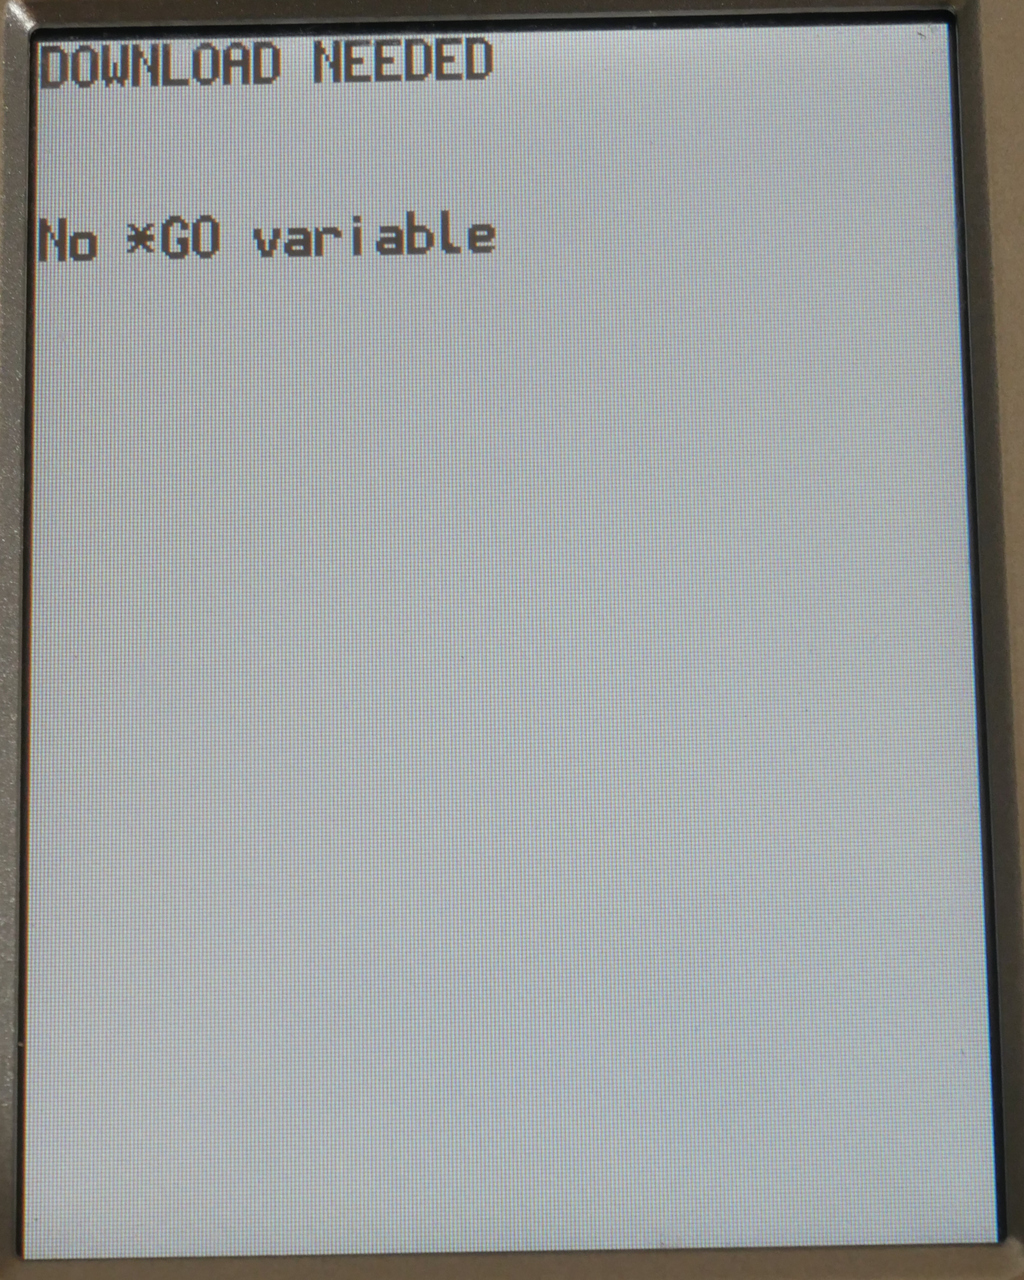
\includegraphics[width=5.5cm]{media/lcd_tamper7}
	\end{column}
\end{columns}
\end{frame}

% 19 minuten voor deze slide

\begin{frame}[fragile]{Getting access}{Downloading applications}
\begin{columns}
	\begin{column}{0.5\textwidth}
		\texttt{DOWNLOAD NEEDED}?
		\begin{itemize}
			\item Proprietary protocol called XDL
			\item Features:
			\begin{itemize}
				\item Load files
				\item Set config variables
				\item Wipe flash or SRAM
			\end{itemize}
		\end{itemize}
	\end{column}
	\begin{column}{0.5\textwidth}
			\pause
			Easily reverse engineered :)

			~

			\begin{minted}{python}
from xdl import XDL

binary = "APP.OUT"

xdl = XDL()

xdl.connect()
xdl.set_config_var("*GO", binary)
xdl.send_file(binary)
xdl.stop()
			\end{minted}
	\end{column}
\end{columns}
~\\~\\
\url{https://github.com/ThomasRinsma/pyxdl}
\end{frame}

% TODO: explain filesystems, .OUT, config vars (*GO)


\begin{frame}{Getting access}
	So, can we just upload \texttt{DOOM.OUT}?
\end{frame}


\begin{frame}{Getting access}{Program authentication}
\begin{columns}
\begin{column}{0.6\textwidth}
	Yes, but...
	\begin{itemize}
		\item Programs (\texttt{.OUT}) normally come with a signature file (\texttt{.P7S})
		\item Replaced with a \texttt{.S1G} file after first boot.
		
		\item On boot: ~\\
		~~~~\texttt{if(verify\_p7s(file))}~\\
		~~~~~~~~\texttt{generate\_s1g(file);}
		

		\item Runtime: ~\\
		~~~~\texttt{verify\_s1g(file);}
	\end{itemize}
~\\
\footnotesize{
Source: research by \href{https://twitter.com/ivachyou}{\texttt{@ivachou}} and \href{https://twitter.com/A1ex_S}{\texttt{@A1ex\_S}}:~\\
\url{https://www.paymentvillage.org/resources}}
\end{column}
\begin{column}{0.4\textwidth}
	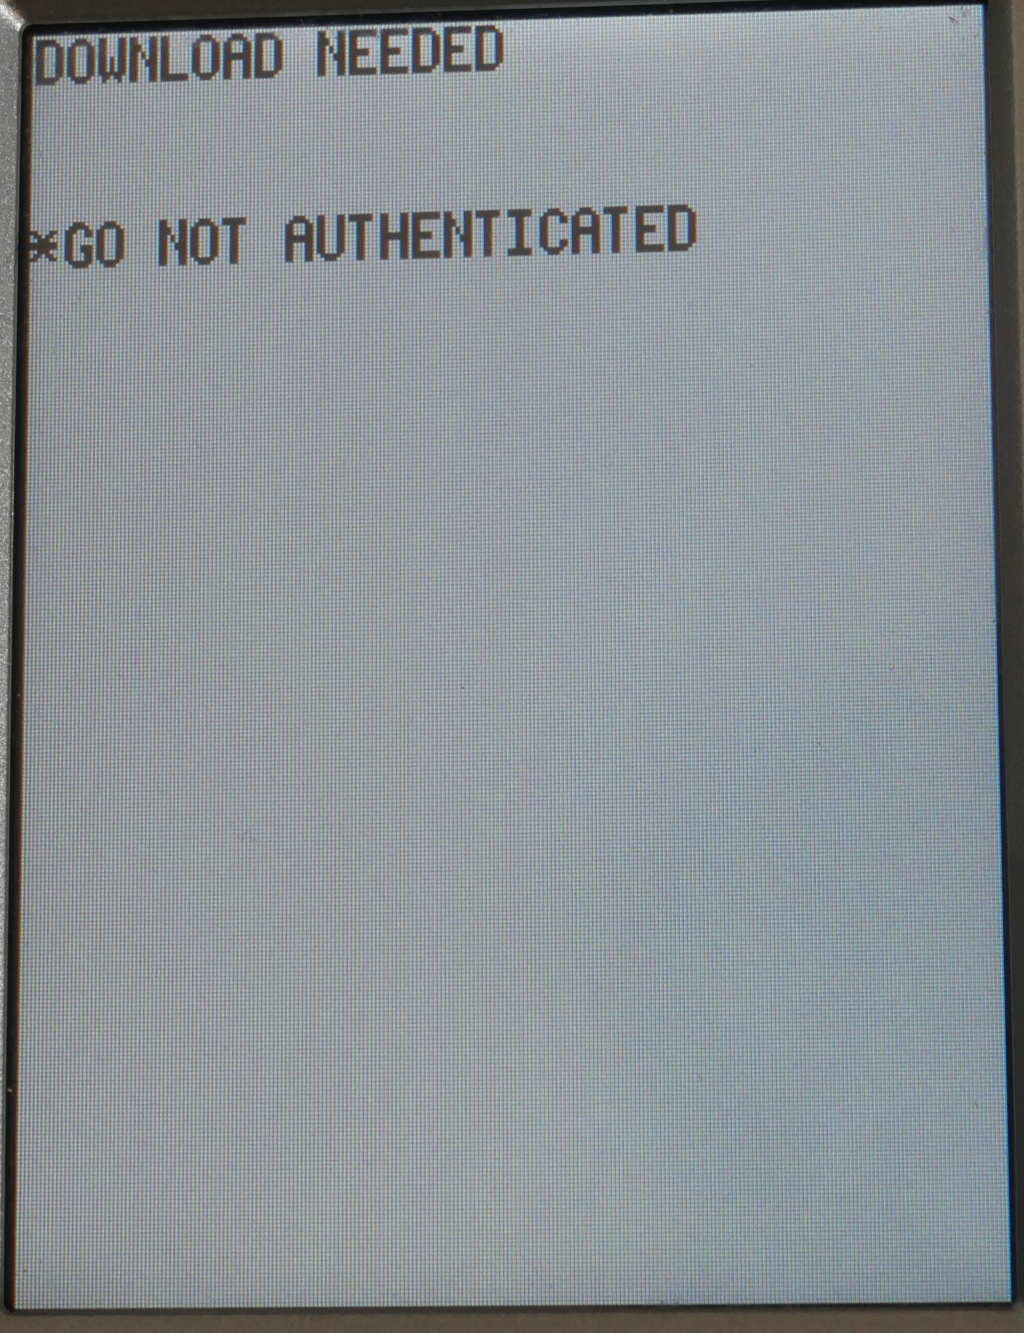
\includegraphics[width=5.5cm]{media/go_not_auth}
\end{column}
\end{columns}
\end{frame}

\begin{frame}{Known issues}
\begin{columns}
	\begin{column}{0.6\textwidth}
		Previously found ``features''/bugs:
		~\\~\\
		\begin{enumerate}
			\item<2-> Hidden shell: \texttt{T:SHELL.OUT}
			\begin{itemize}
				\item<2-> interesting but low privilege
			\end{itemize}
			\item<3-> Buffer overflow in kernel code
			\begin{itemize}
				\item<3-> patched or different per OS version
			\end{itemize}
			\item<4-> Hidden bootloader mode
			\begin{itemize}
				\item \textbf{Still present in this device!} 
			\end{itemize}
		\end{enumerate}
		~\\~\\
		\footnotesize{
		Source: research by \href{https://twitter.com/ivachyou}{\texttt{@ivachou}} and \href{https://twitter.com/A1ex_S}{\texttt{@A1ex\_S}}:~\\
		\url{https://www.paymentvillage.org/resources}}
	\end{column}
	\begin{column}{0.4\textwidth}
		\includegraphics<2>[width=5cm]{media/vx820_shell}
		\includegraphics<4>[width=8cm]{media/sbi_uart}
	\end{column}
\end{columns}
\end{frame}


\begin{frame}{Boot sequence}{Overview}
\begin{columns}
	\begin{column}{\textwidth}
		\begin{itemize}
			\item ``Secure boot'': each stage authenticates the next
			\item 2nd stage (SBI) authenticates and loads Verix OS
			\item SBI also listens for a keycombo: \textbf{1}+\textbf{5}+\textbf{9}
			\begin{itemize}
				\item Uses XDL to load authenticated \emph{scripts}
				\item Or, if a magic header is provided: \\
				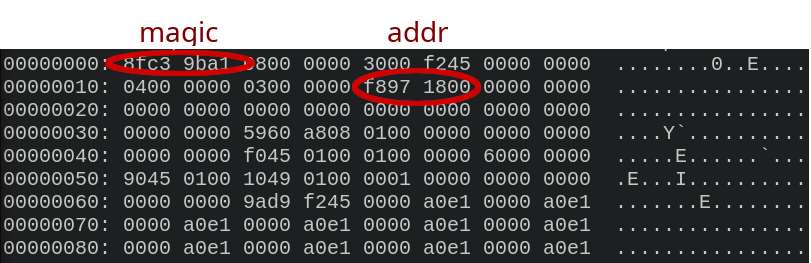
\includegraphics[width=8cm]{media/sbi_magic.png} \\
				\texttt{memcpy(addr, file\_contents, file\_len)}
			\end{itemize}

		\end{itemize}
	\end{column}
	% \begin{column}{0.3\textwidth}
	% 	TODO: diagram of boot sequences
	% \end{column}
\end{columns}
\end{frame}

% 	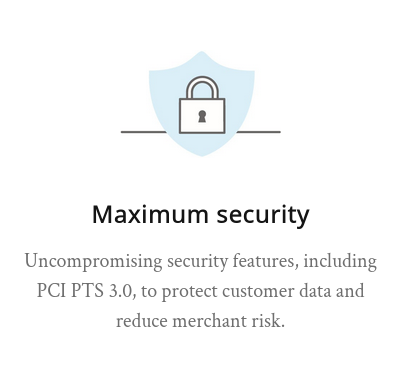
\includegraphics[width=0.8\textwidth]{media/maximum_security}


% \begin{frame}{Boot sequence}{Previous research}
% 	\centering
% 	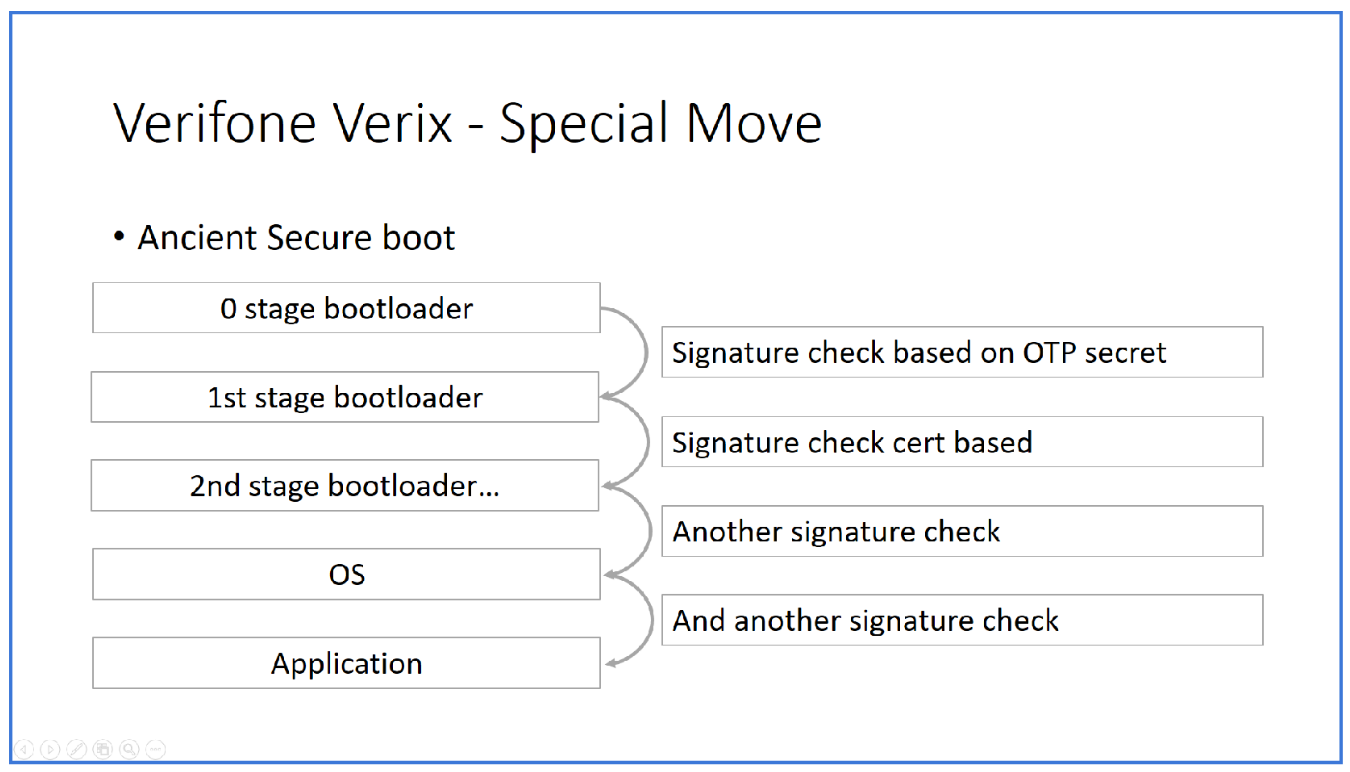
\includegraphics[width=0.7\textwidth]{media/boot_flow_posworld}~\\
% 	\footnotesize{Source: ``POSWorld'', Payment Village}
% \end{frame}

\begin{frame}{Boot sequence}{Summary}
\begin{columns}
	\begin{column}{0.5\textwidth}
		To summarize:

		\begin{itemize}
			\item<1-> Arbitrary write allows for code execution
			\item<1-> Completely breaking secure boot
			\item<2-> Somehow still present on these devices!

			~

			\item<3-> Luckily for us: this is a way in :)
		\end{itemize}
	\end{column}
	\begin{column}{0.5\textwidth}
	\includegraphics<2->[width=\textwidth]{media/sbi_versions}
	\end{column}
\end{columns}
\end{frame}


\begin{frame}{Code execution}{The plan}
Use code execution in SBI to get control over Verix:
\begin{enumerate}
	\item Overwrite SBI with a patched version
	\item Keep original bootloader functionality intact
	\item Add a patch to the OS that calls ~ \texttt{gen\_s1g("H.OUT");}
\end{enumerate}
\end{frame}



\begin{frame}{Code execution (1)}
\vspace{-1.5mm}
\only<1>{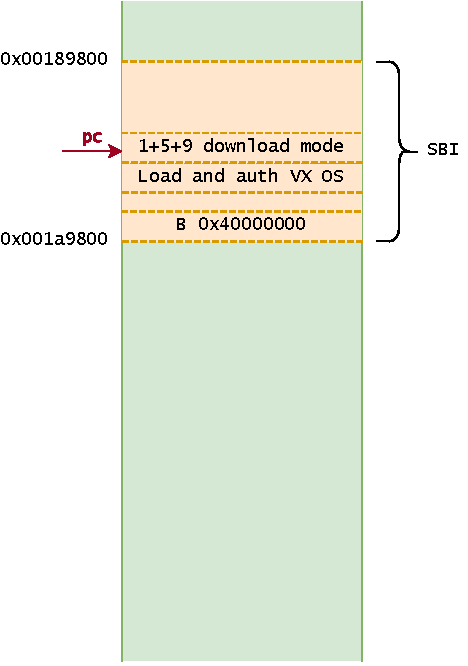
\includegraphics[height=8cm]{media/vx820_boot_flow_1}}
\only<2>{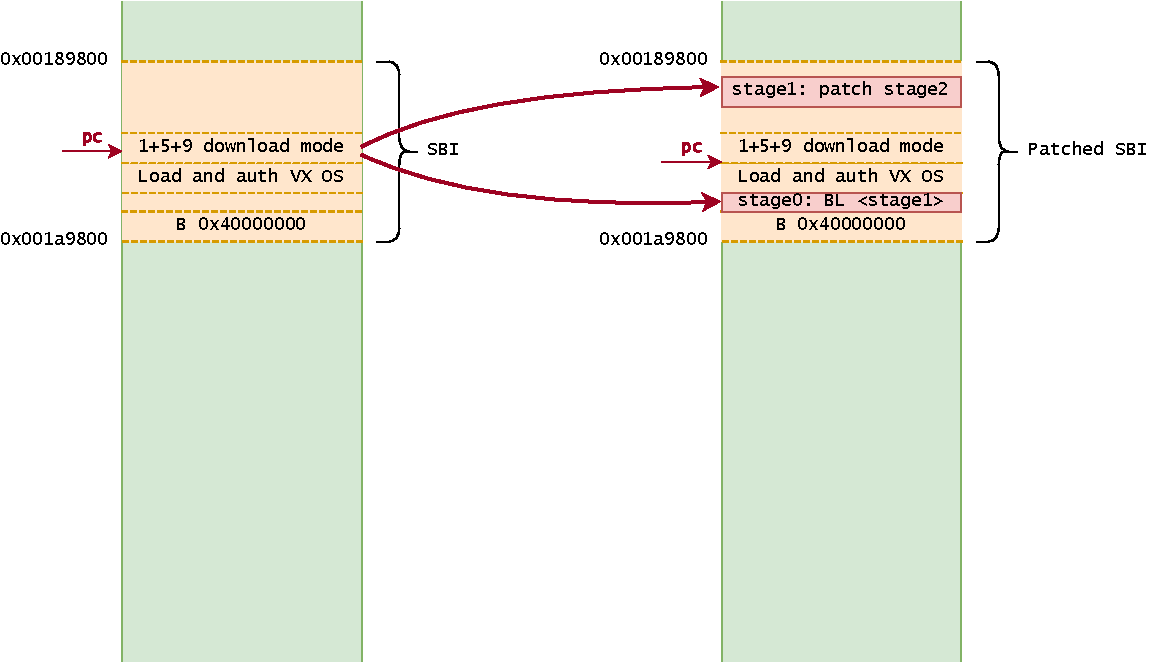
\includegraphics[height=8cm]{media/vx820_boot_flow_2}}
\end{frame}

\begin{frame}{Code execution (2)}
\vspace{-1.5mm}
\only<1>{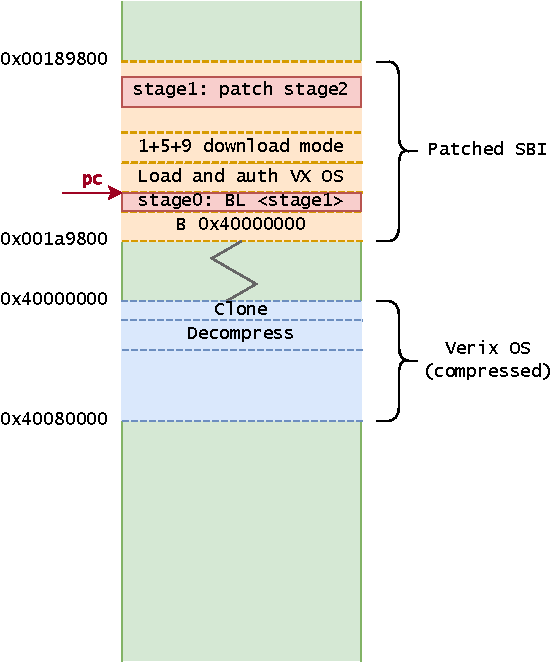
\includegraphics[height=8cm]{media/vx820_boot_flow_3}}
\only<2>{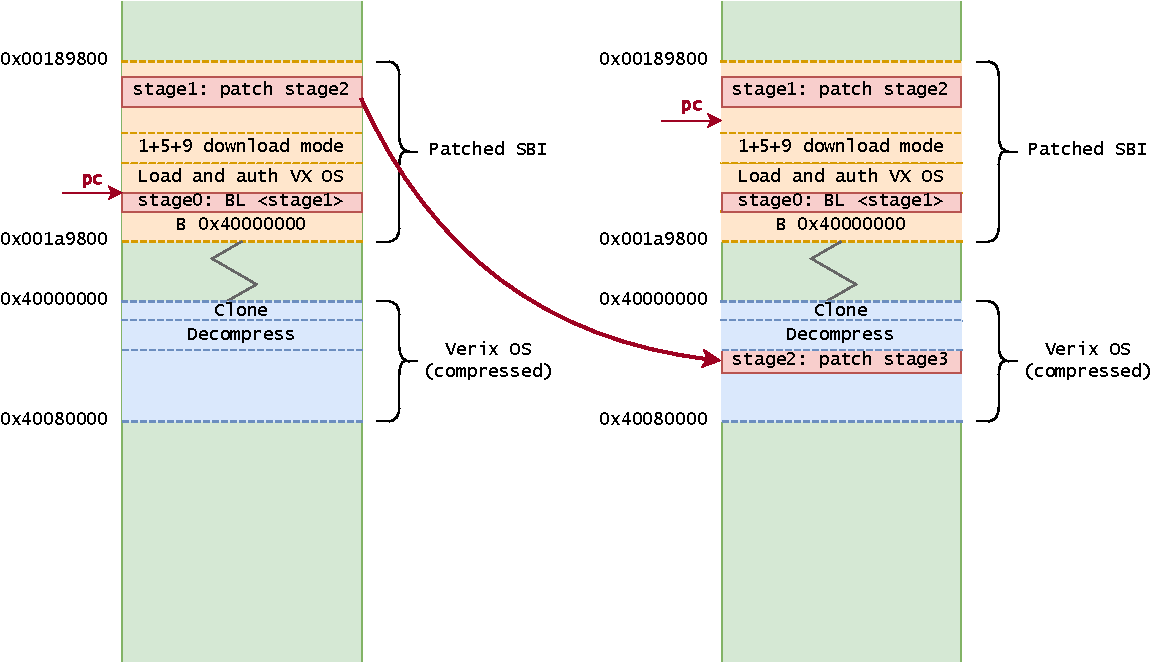
\includegraphics[height=8cm]{media/vx820_boot_flow_4}}
\end{frame}

\begin{frame}{Code execution (3)}
\vspace{-1.5mm}
\only<1>{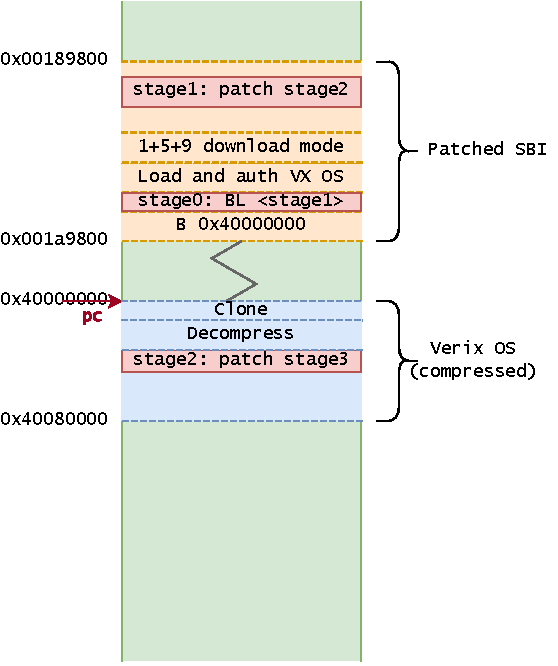
\includegraphics[height=8cm]{media/vx820_boot_flow_5}}
\only<2>{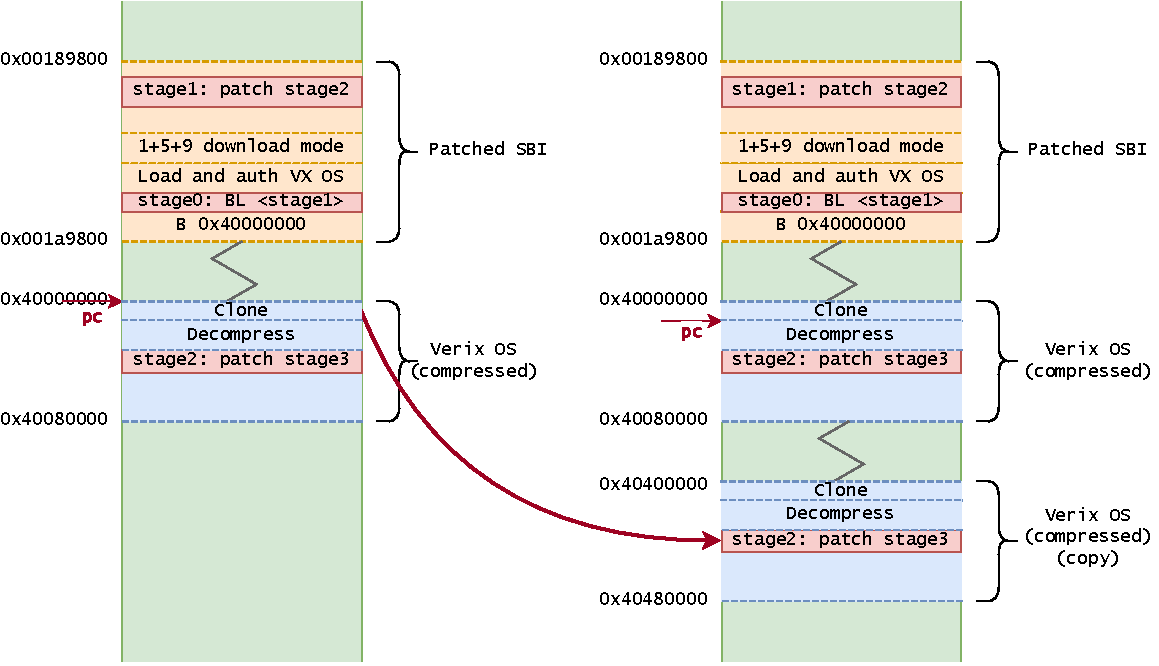
\includegraphics[height=8cm]{media/vx820_boot_flow_6}}
\end{frame}

\begin{frame}{Code execution (4)}
\vspace{-1.5mm}
\only<1>{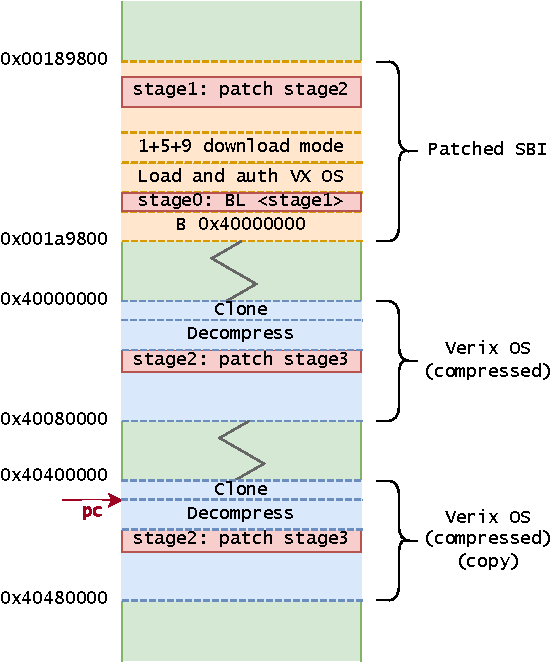
\includegraphics[height=8cm]{media/vx820_boot_flow_7}}
\only<2>{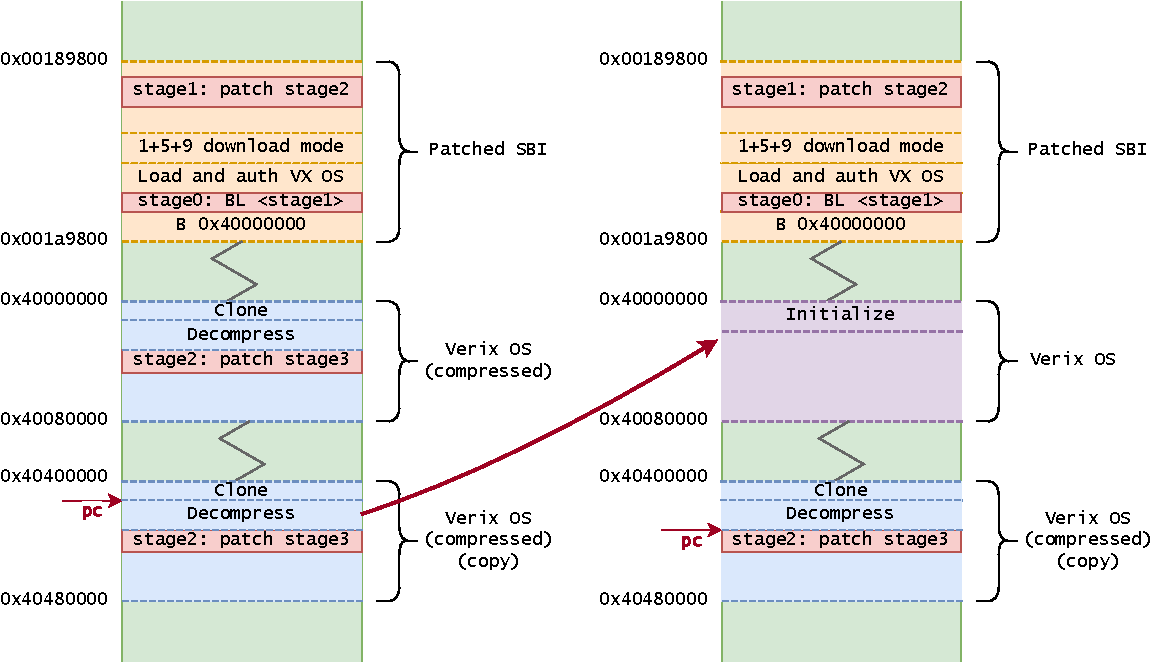
\includegraphics[height=8cm]{media/vx820_boot_flow_8}}
\end{frame}

\begin{frame}{Code execution (5)}
\vspace{-1.5mm}
\only<1>{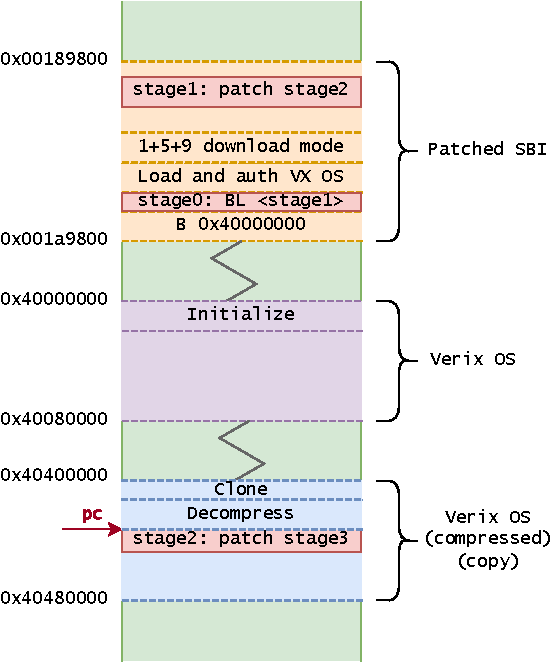
\includegraphics[height=8cm]{media/vx820_boot_flow_9}}
\only<2>{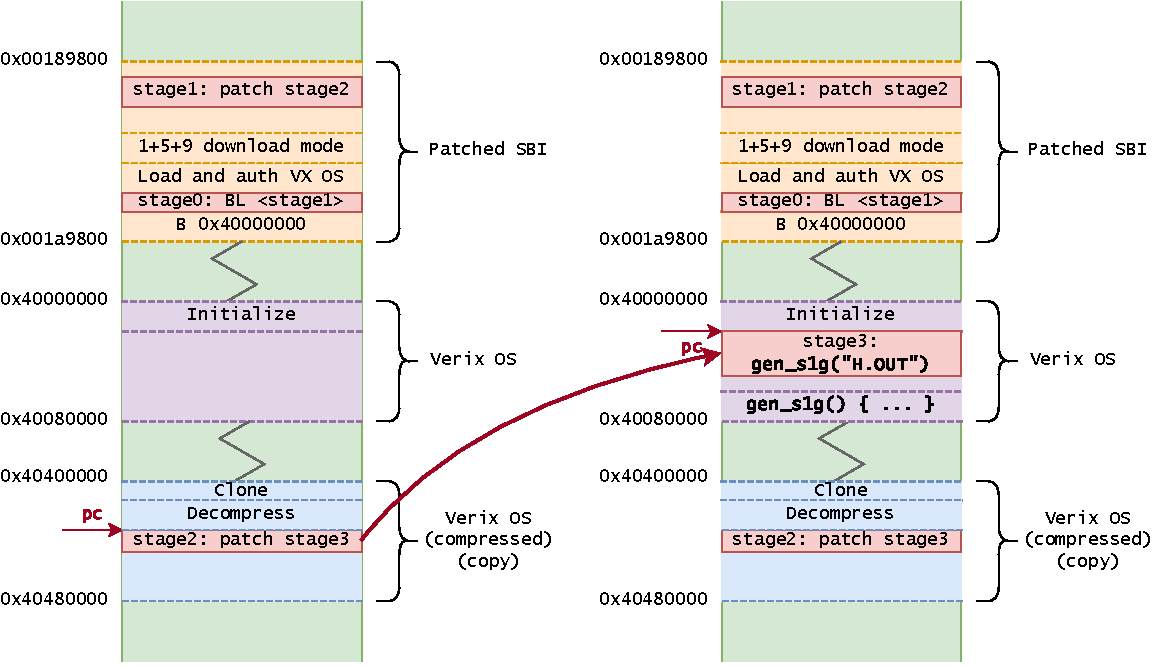
\includegraphics[height=8cm]{media/vx820_boot_flow_10}}
\end{frame}

\begin{frame}{Code execution}{The result}
\centering
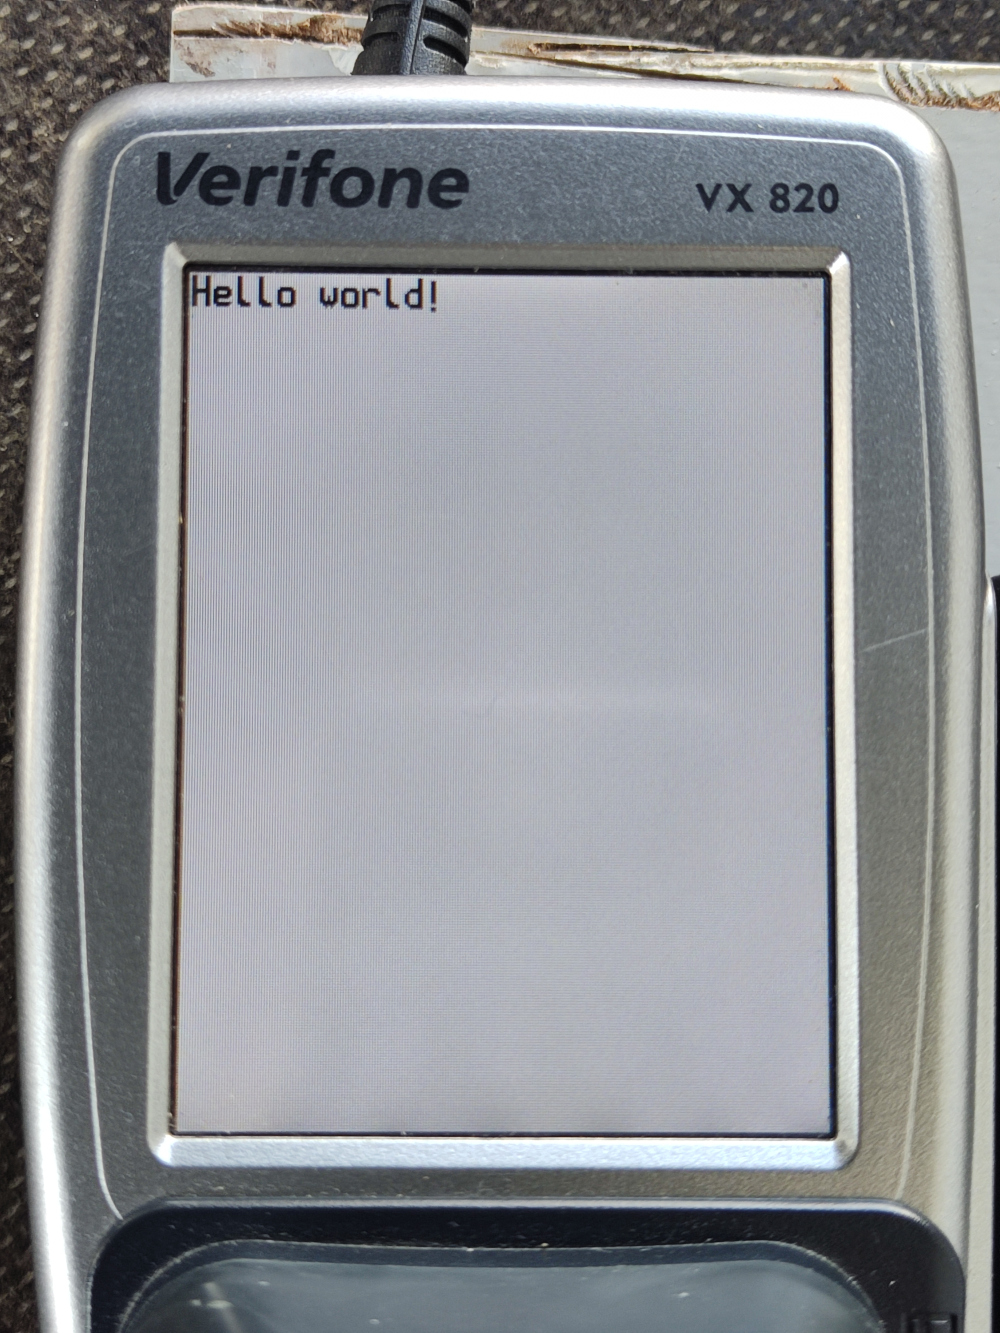
\includegraphics[height=10cm]{media/vx820_hello_world}
\end{frame}

\begin{frame}{Executable format}
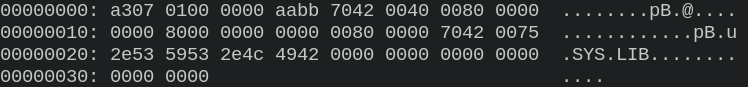
\includegraphics[width=\textwidth]{media/executable_format_xxd}
The program header specifies:
~\\
\begin{itemize}
	\item Magic and various flags (?)
	\item Entrypoint
	\item Which system libraries to load (e.g. \texttt{SYS.LIB})
	\item Start and size of code (ELF's \texttt{.text})
	\item Size of read-only data (ELF's \texttt{.rodata})
	\item Stack size
\end{itemize}
\end{frame}

\begin{frame}{Toolchain}
\begin{columns}
	\begin{column}{0.5\textwidth}
		Format seems pretty simple!

		\pause
		~\\
		Let's make a hacky ``toolchain'':
		\begin{itemize}
			\item Build an ARMv6 ELF file normally
			\item Extract the relevant sections
			\item Copy-paste the header and patch the sizes
		\end{itemize}
	\end{column}
	\begin{column}{0.5\textwidth}
		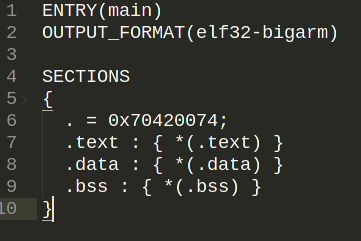
\includegraphics[width=5cm]{media/linker_script}\\
		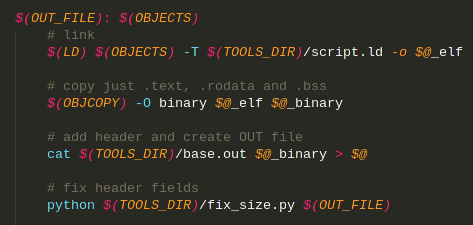
\includegraphics[width=7cm]{media/hacky_toolchain}
	\end{column}
\end{columns}
\end{frame}


\begin{frame}{Toolchain}{Syscalls}
We want to be able to print to the screen, read input, etc.~\
$\longrightarrow$ \textbf{syscalls}.
~\\~\\
\begin{itemize}
	\item The interface is familiar: \texttt{open}, \texttt{read}, \texttt{write}, etc.
	\begin{itemize}
		\item print to screen: \texttt{write} to \texttt{/DEV/CONSOLE}
		\item read keystrokes: \texttt{read} from \texttt{/DEV/CONSOLE}
	\end{itemize}
	\item Syscall numbers can be RE'd from other programs and public documentation
\end{itemize}
\end{frame}



\begin{frame}{Toolchain}
Now it's a matter of engineering: \\~\\
\begin{columns}
	\begin{column}{0.33\textwidth}
		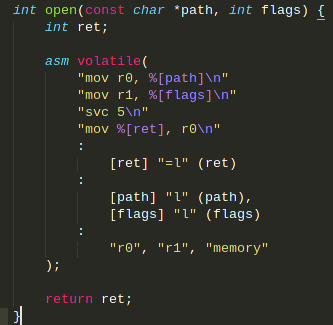
\includegraphics[width=\textwidth]{media/syscall_open}
	\end{column}
	\begin{column}{0.33\textwidth}
		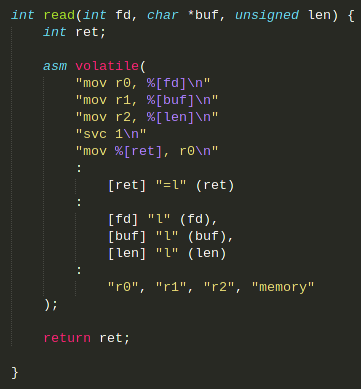
\includegraphics[width=\textwidth]{media/syscall_read}
	\end{column}
	\begin{column}{0.33\textwidth}
		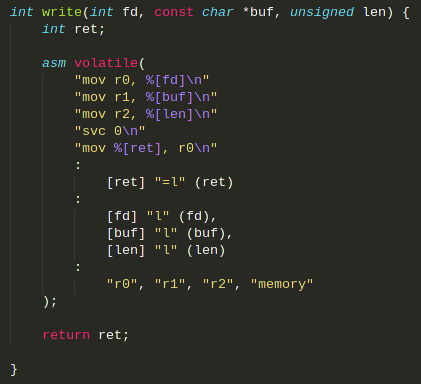
\includegraphics[width=\textwidth]{media/syscall_write}
	\end{column}
\end{columns}
~\\
etcetera...
\end{frame}



\begin{frame}{Porting stuff}
	\emph{Now} we can start porting Doom :)
	~\\~\\~\\
	\large
	\centering
	[ demo time ]
\end{frame}

\begin{frame}{The end}
\centering
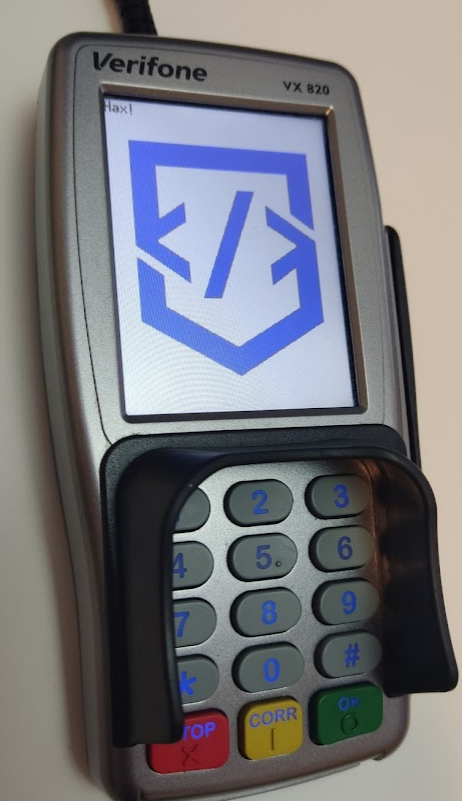
\includegraphics[width=0.15\textwidth]{media/codean_logo}
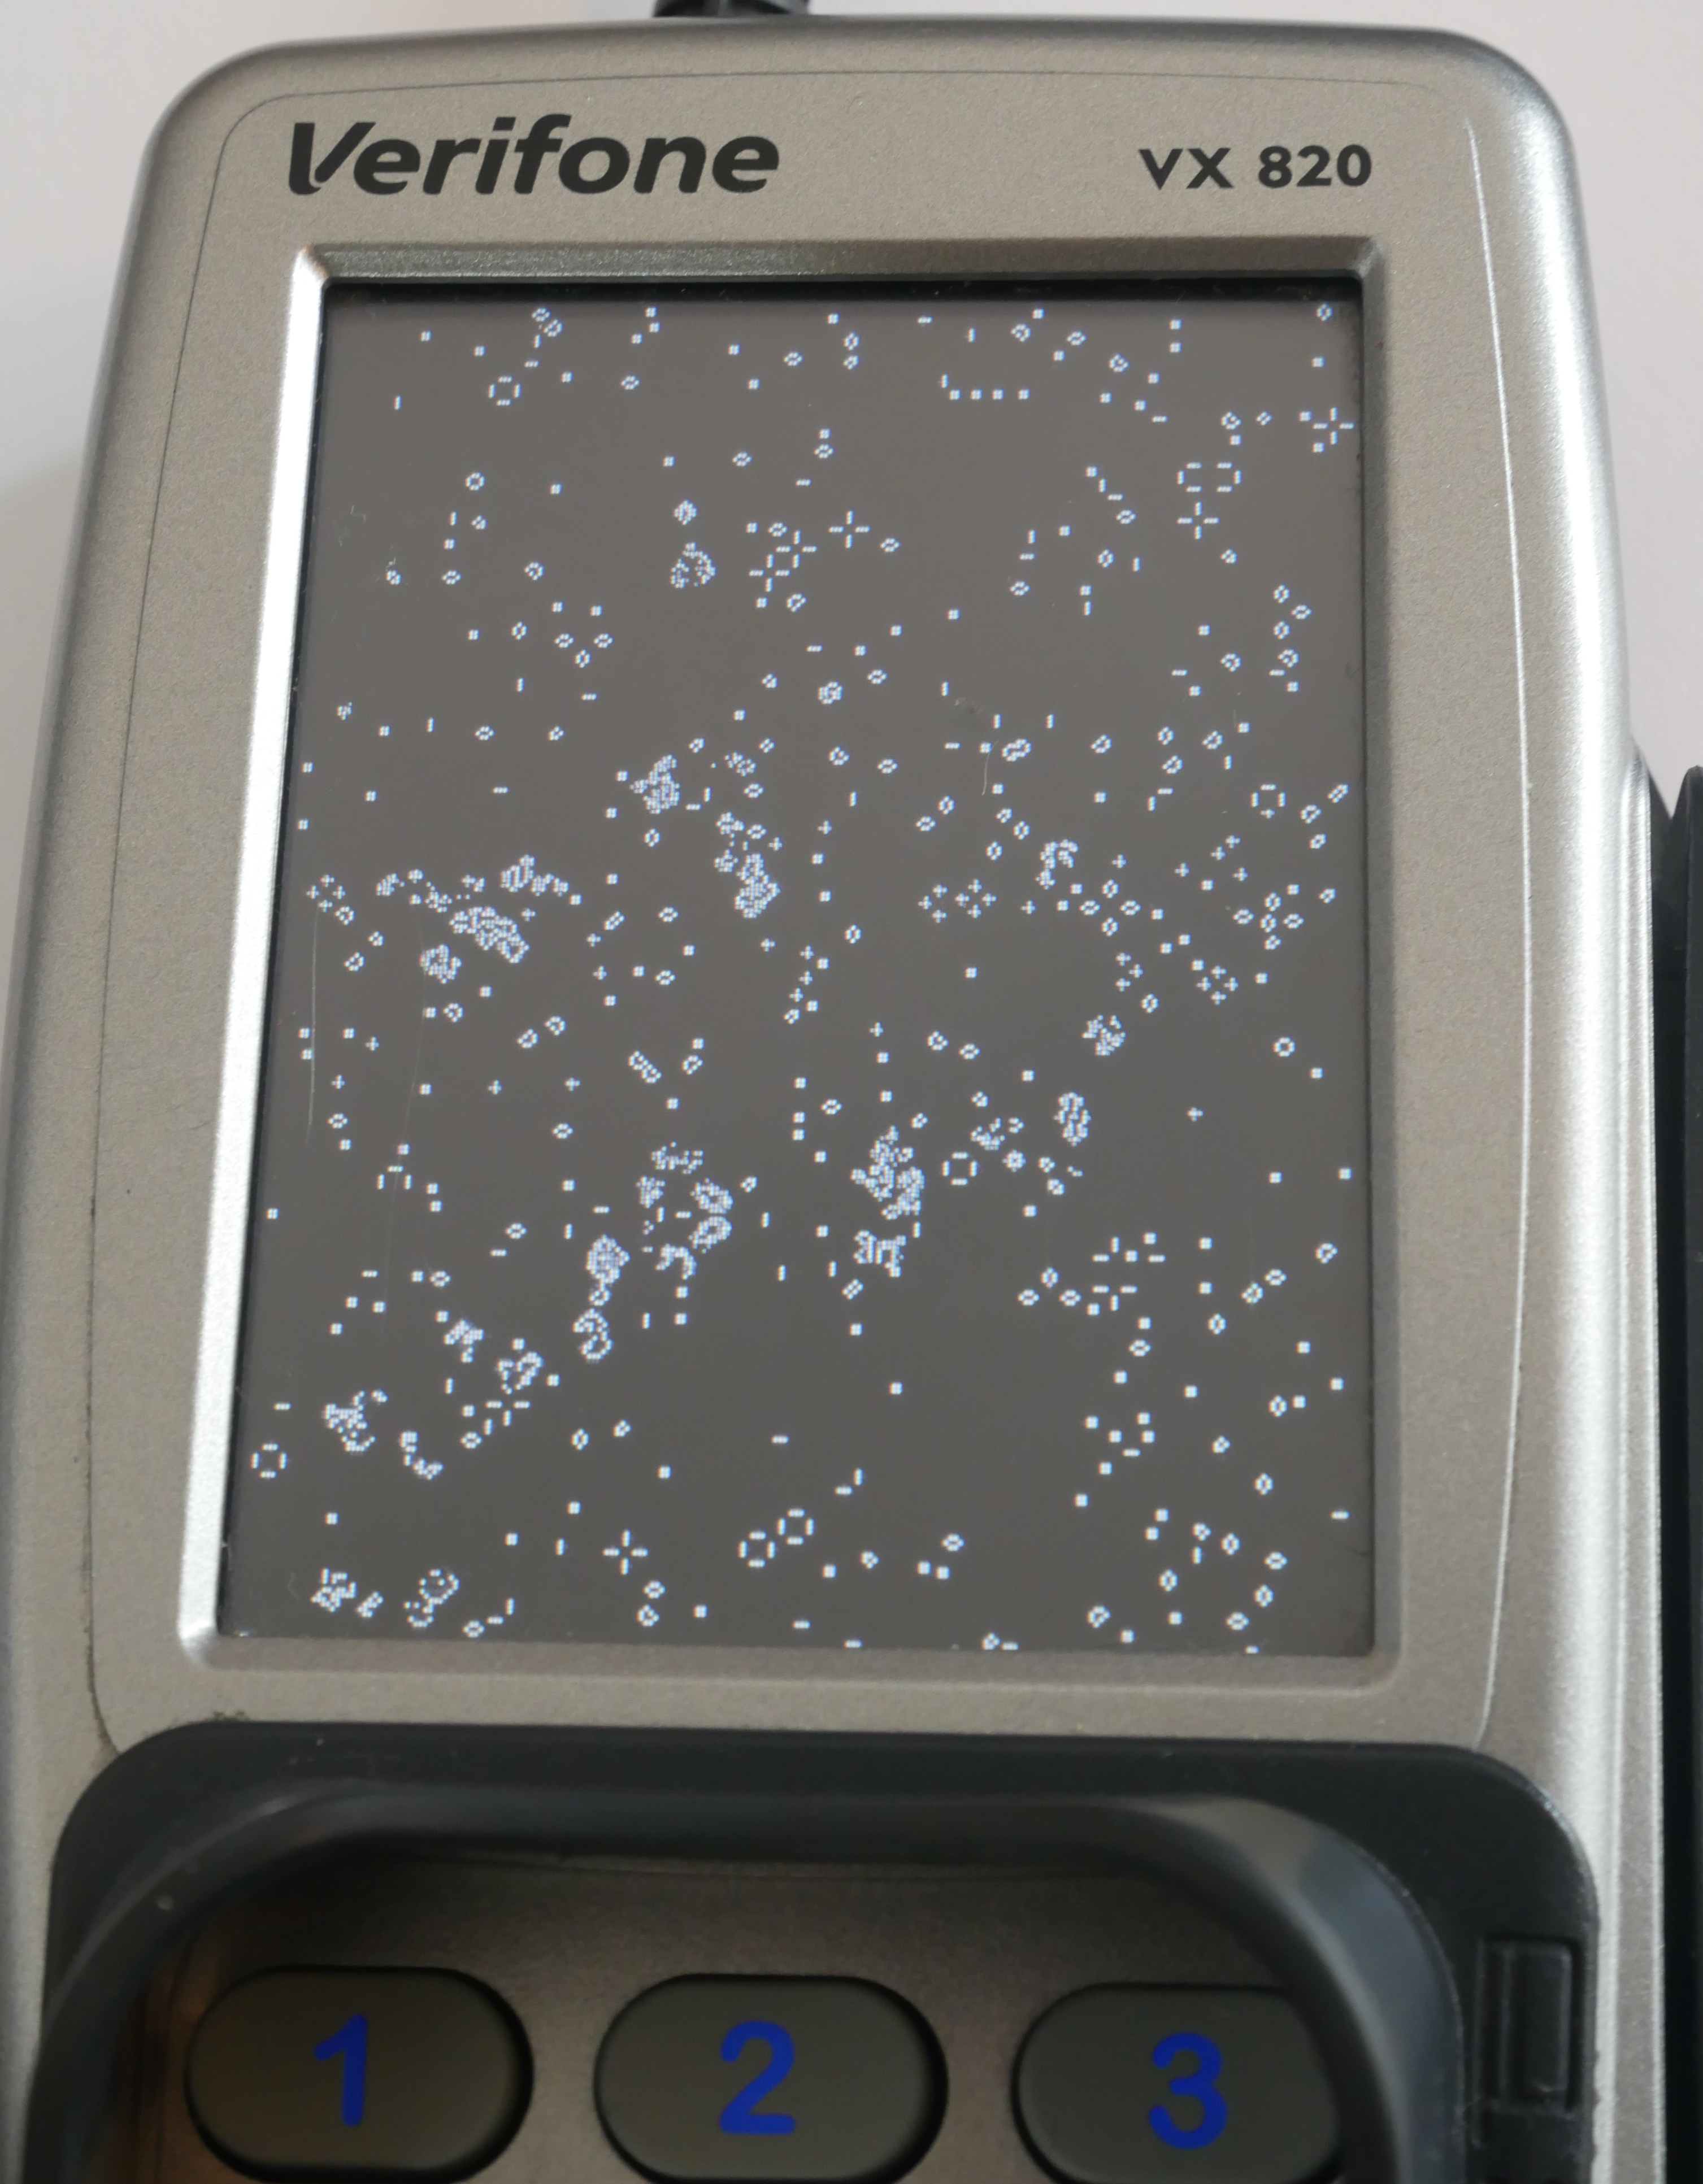
\includegraphics[width=0.25\textwidth]{media/gol}
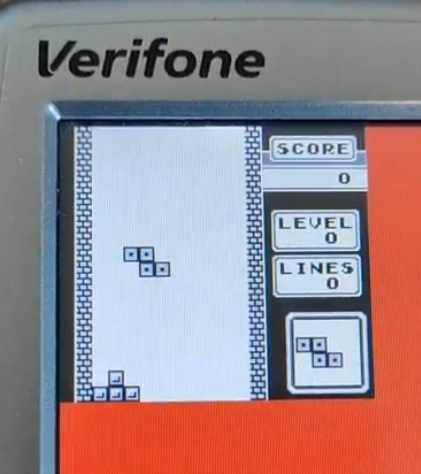
\includegraphics[width=0.25\textwidth]{media/gb_tetris}
% 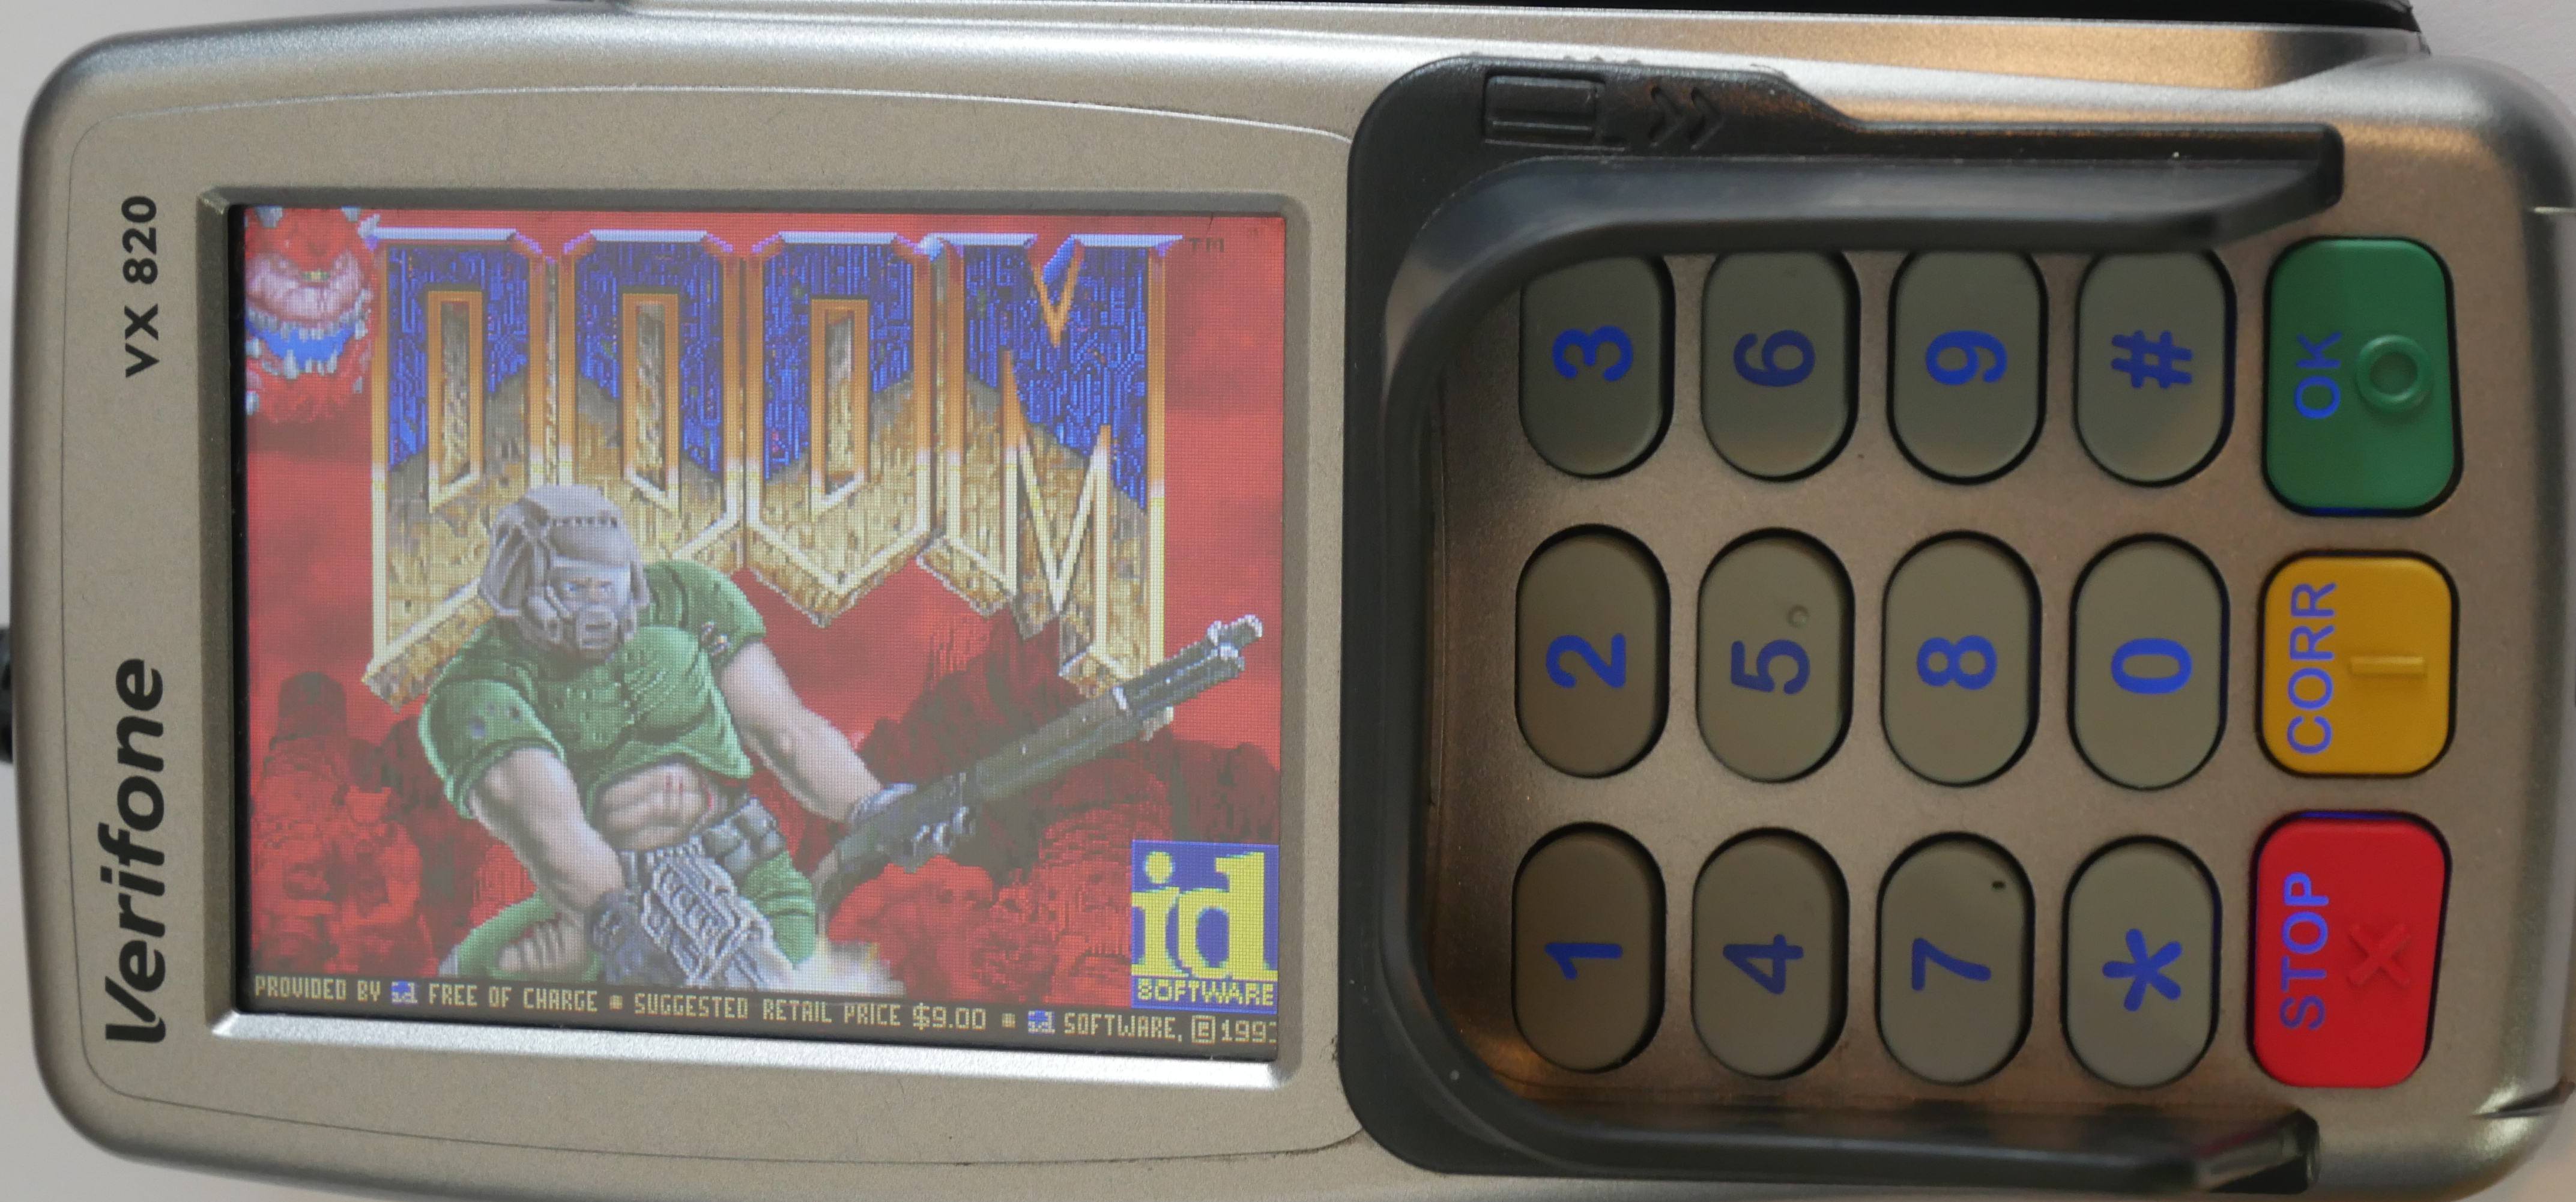
\includegraphics[width=0.29\textwidth]{media/doom}
~\\~\\
\href{https://twitter.com/thomasrinsma}{\texttt{@thomasrinsma}}\\
\url{https://th0mas.nl/2022/07/18/verifone-pos-hacking/}
\end{frame}

% \item Operating system
% 	% - General architecture
% 	% - Syscall API
% 	% - How it is loaded / it loads itself

% \item Building a "toolchain"
% 	% - Proprietary binary format
% 	% - difficulty with .data
% 	% - hacky libc

% \item Porting Doom and more
% 	% - Doom is perfect for this: does only one malloc
% 	% - Learned about display scaling / mode 13(?)

% \item Demo time



% \begin{frame}
% \frametitle{Building a ``toolchain''}

% \begin{columns}
% 	\begin{column}{0.5\textwidth}
% 		\begin{itemize}
% 			\item Binary format is proprietary, but simple enough.
% 			\item Managed to hack something by concatenating ELF sections.
% 			\begin{itemize}
% 				\item .bss but no .data...
% 			\end{itemize}
% 		\end{itemize}
% 	\end{column}
% 	\begin{column}{0.5\textwidth}
% 		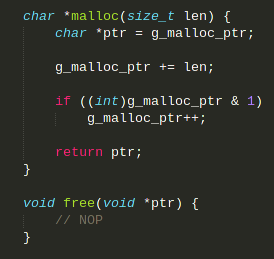
\includegraphics[width=0.45\textwidth]{media/malloc_free}
% 		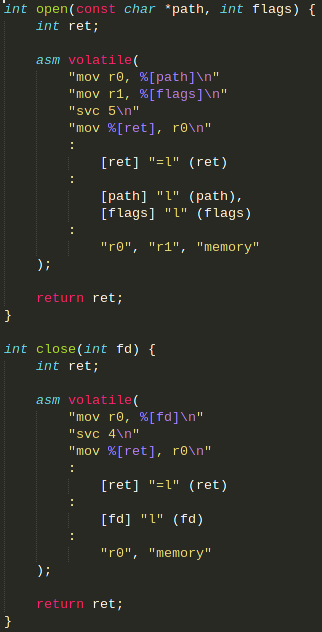
\includegraphics[width=0.45\textwidth]{media/syscalls}
% 	\end{column}
% \end{columns}
% \end{frame}


% \begin{frame}
% \frametitle{The end! (but the fun begins)}
% \centering
% \includegraphics[width=0.1\textwidth]{media/codean_logo}
% \includegraphics[width=0.25\textwidth]{media/gol}
% \includegraphics[width=0.25\textwidth]{media/gb_tetris}
% \includegraphics[width=0.6\textwidth]{media/doom}


% \end{frame}

\end{document}